%\documentclass[12pt,twocolumn]{article}
\documentclass[12pt]{article}
\usepackage[utf8]{inputenc}
\usepackage{amsmath}
\usepackage{listings}
\usepackage{graphicx}
\usepackage{verbatim}
\title{CS 472 Fall 2011 \\
     Project 1}
\author{Colby Blair}
\date{Due September 28th, 2011}

\begin{document}
\maketitle

\begin{abstract}
Evolutionary Computation is the study of combonational logic, that can often provide reasonable solutions to
intractably complex problems. In Evolutionary Computation, there are many different approaches to optimizing a solution for a problem. Different approaches often result in better result, depending on the problem to be solved. This project considers the Spherical, Rosenbrock, Rastrigin, Schwefel, Ackley, and Griewangk functions, and tries to optimize parameters for them using a Genetic Algorithm (GA).

This report finds that the functions rank easiest to hardest to optimize as Ackley, Spherical, Griewangk, Rosenbrock, Rastrigin, and Schwefel. Ease of optimization is judged on how close to optimizing the GA gets, and how many generations it takes. For most, they are limited to 10000 generations maximum. Each test is run multiple times, and the results are similar.
\end{abstract}
\pagebreak

\part{Algorithm Descriptions}
\label{part:alg_desc}

A Genetic Algorithm (GA) creates a \textbf{population} of individuals, each of which have attributes to try to solve a problem. Their correctness will be measure with a \textbf{fitness function}. The best of these individuals are found with \textbf{selection}, their attributes are combined using \textbf{crossover}, and a child is produced from this. Each child is then slightly \textbf{mutated}, or its attributes changed. This results in new individuals in the population, and the whole process is started again.

The \textbf{population} for all the GA methods in this report is represented as a list of vectors. The \textbf{initial population} has random values set in the attributes vector (x) for every individual (see Figure \ref{uniform_mutation}):
\begin{figure}[!h]
        \begin{center}
		\begin{tabular}{r l}
	                $ P = i_1, i_2, ... i_j $	& \\
								& where \\
								& $ i_n $ is a vector of floats or integers ( $ = x_1, x_2, ... x_y $ ) \\
								& $ j = 500 $ \\
								& $ y = 30 $ \\
								& $ x_n = [B_L, B_U] $ \\
								& $ B_L $ is the lower bound, specified by each function\\
								& $ B_U $ is the upper bound, specified by each function\\
		\end{tabular} 
               \caption{The representation of the population}
                \label{population}
        \end{center}
\end{figure}

The GA methods here will use the each function to calculate their \textbf{fitness} (refer to each of the following \textbf{function description} sections in Section \ref{part:func_defs}). The GA's will then try to find the minimum fitnesses, or the individual(s), that calculate to the minimum.

For \textbf{selection} (Figure \ref{selection}), the two individuals with the smallest fitnesses (best) will be selected from a random sample of the entire population. The sample size is represented by $ k $. As $ k $ gets bigger, the best individuals of a population are more likely preserved, while $ k $ getting smaller means more variety in the population. 
\begin{figure}[!h]
        \begin{center}
		\begin{tabular}{r l}
			$ selection(P) = $		&	$ i_1, i_2, ... i_k$ \\
								& \\
								&	where \\
								&	$ P $ is the entire population \\
								&	$ i_k $ is a random individual \\
								&	$ k $ is the sample size, specified at run time \\
		\end{tabular} 
               \caption{The selection function}
                \label{selection}
        \end{center}
\end{figure}

Generally, $ k $ being larger leads to conversion on local optimums that the population may be surrounding, while $ k $ being lower allows individuals that may lead to some other optimum to remain. With functions like the spherical function, there is only one global / local minimum, so $ k $ should be set high.

The \textbf{crossover} function will take two individuals $ i_a, i_b $, and return a child individual, which has a mix of attributes ( $x_n $ values) from each parent. Specifically, \textbf{one point crossover} is used:
\begin{figure}[!h]
        \begin{center}
		\begin{tabular}{r l}
	                $ crossover(i_a, i_b) = $ & \\
			& $ x_{i_a}[1:n], x_{i_b}[n + 1:length(i_b)] $ x values for the new child individual \\
								& where \\
								& $ n = $ a random integer from $ 1 ... $ the length of $ i_a $ or $ i_b$ (same)
		\end{tabular} 
               	\caption{One point crossover}
                \label{one_crossover}
        \end{center}
\end{figure}

Finally, an alteration of the \textbf{creep mutation} function was used. For any new child created from crossover, all of its attributes would then be mutated a little bit before insertion into a new population. :

\begin{figure}[!h]
        \begin{center}
		\begin{tabular}{r l}
	                $ mutate(x_i) $ 		& $ = x_{i}{'}[1,2, ... n] $  \\
								& where \\
								& $ x_{i}{'}[m] = D * S $\\
								& $ D = x_{i}{'}[m] - R $ \\
								& $ R $ is a random value from $ B_L $ to $ B_U $ \\ 
								& $ S $ is a scaling factor, $ = .10 $ \\
								& $ n = $ length of $x_i$ \\
								& $ m = 1,2,...n$ \\
		\end{tabular} 
               	\caption{Creep mutation}
                \label{creep_mutation}
        \end{center}
\end{figure}


\section{Steady State}
The \textbf{steady state} algorithm used the \textbf{population} described in Figure \ref{population}, the \textbf{fitness} function described in Figure \ref{fitness}, the \textbf{selection} described in Part \ref{part:alg_desc}, the \textbf{crossover} described in Figure \ref{one_crossover}, and the \textbf{mutation} described in Figure \ref{uniform_mutation}.

The flow of converging on a solution is as follows:
\begin{itemize}
	\item while min fitness of population is greater than 0.00
	\begin{itemize}
		\item calculate current fitnesses
		\item select 2 individuals (parents) with minimum fitnesses
		\item create new child from the 2 parents using one point crossover
		\item mutate the new child using uniform mutation
		\item replace the individual in the population with the max fitness, with the new child
	\end{itemize}
\end{itemize}


\part{Function Descriptions}
\label{part:func_defs}

\section{Spherical Function}
\begin{figure}[!h]
        \begin{center}
		\begin{tabular}{r l}
			$ f_{Sph}(i_j) = $			&	$ \sum_{i=1}^{1}x_i^2 $ \\
								& \\
								&	where \\
								&	$ i_j $ is an individual \\
								&	$ x_i = [B_L, B_U] $ \\
								& $ B_L $ is the lower bound, $ = -5.12 $\\
								& $ B_U $ is the upper bound, $ = 5.12 $\\

		\end{tabular} 
               \caption{The spherical function}
                \label{spherical}
        \end{center}
\end{figure}

\pagebreak

\section{Rosenbrock Function}
\begin{figure}[!h]
        \begin{center}
		\begin{tabular}{r l}
			$ f_{Ros}(i_j) = $		&	$ \sum_{i=1}^{p-1} [100 (x_{i+1} - x_{i}^{2})^2 + (x_i - 1)^2] $ \\
								& \\
								&	where \\
								&	$ x_i = [B_L, B_U] $ \\
								& 	$ B_L $ is the lower bound, $ = -2.048 $\\
								& 	$ B_U $ is the upper bound, $ = 2.048 $\\

		\end{tabular} 
               \caption{The Rosenbrock function}
                \label{rosenbrock}
        \end{center}
\end{figure}

\section{Rastrigin Function}
\begin{figure}[!h]
        \begin{center}
		\begin{tabular}{r l}
			$ f_{Ras}(i_j) = $		&	$ 10p + \sum_{i=1}^{1} (x_i^2 - 10 cos(2\pi x_i) )$ \\
								& \\
								&	where \\
								&	$ x_i = [B_L, B_U] $ \\
								& 	$ B_L $ is the lower bound, $ = -5.12 $\\
								& 	$ B_U $ is the upper bound, $ = 5.12 $\\

		\end{tabular} 
               \caption{The Rastrigin function}
                \label{rastrigin}
        \end{center}
\end{figure}

\pagebreak

\section{Schwefel Function}
\begin{figure}[!h]
        \begin{center}
		\begin{tabular}{r l}
			$ f_{Sch}(i_j) = $		&	$  418.9829p + \sum_{i=1}^{p} x_i sin(\sqrt{|{x_i}|}) $\\
								& \\
								&	where \\
								&	$ x_y = [B_L, B_U] $ \\
								& 	$ B_L $ is the lower bound, $ = -512.03 $ \\
								& 	$ B_U $ is the upper bound, $ = 511.97 $\\

		\end{tabular} 
               \caption{The Schwefel function}
                \label{schwefel}
        \end{center}
\end{figure}

\section{Ackley Function}
\begin{figure}[!h]
        \begin{center}
		\begin{tabular}{r l}
			$ f_{Ack}(i_j) = $		&	$ 20 + e - 20 e^{ -.2 \sqrt{ \frac{1}{p} \sum_{i=1}^{p} x_i^2 } } - e^{ \frac{1}{p} \sum_{i=1}^{p} cos(2 \pi x_i) }  $\\
								& \\
								&	where \\
								&	$ i_j $ is an individual \\
								&	$ x_i = [B_L, B_U] $ \\
								& 	$ B_L $ is the lower bound, $ = -30 $ \\
								& 	$ B_U $ is the upper bound, $ = 30 $\\

		\end{tabular} 
               \caption{The Ackley function}
                \label{ackley}
        \end{center}
\end{figure}

\pagebreak

\section{Griewangk Function}
\begin{figure}[!h]
        \begin{center}
		\begin{tabular}{r l}
			$ f_{Ack}(i_j) = $		&	$ 1 + \sum_{i=1}^{p} \frac{x_i^2}{4000} - \prod_{i=1}^{p} cos(\frac{x_i}{\sqrt{i}}) $\\
								& \\
								&	where \\
								&	$ i_j $ is an individual \\
								&	$ x_i = [B_L, B_U] $ \\
								& 	$ B_L $ is the lower bound, $ = -30 $ \\
								& 	$ B_U $ is the upper bound, $ = 30 $\\

		\end{tabular} 
               \caption{The Griewangk function}
                \label{griewangk}
        \end{center}
\end{figure}


\pagebreak

\part{Results}

\section{Spherical}
\begin{figure}[!h]
        \begin{center}
		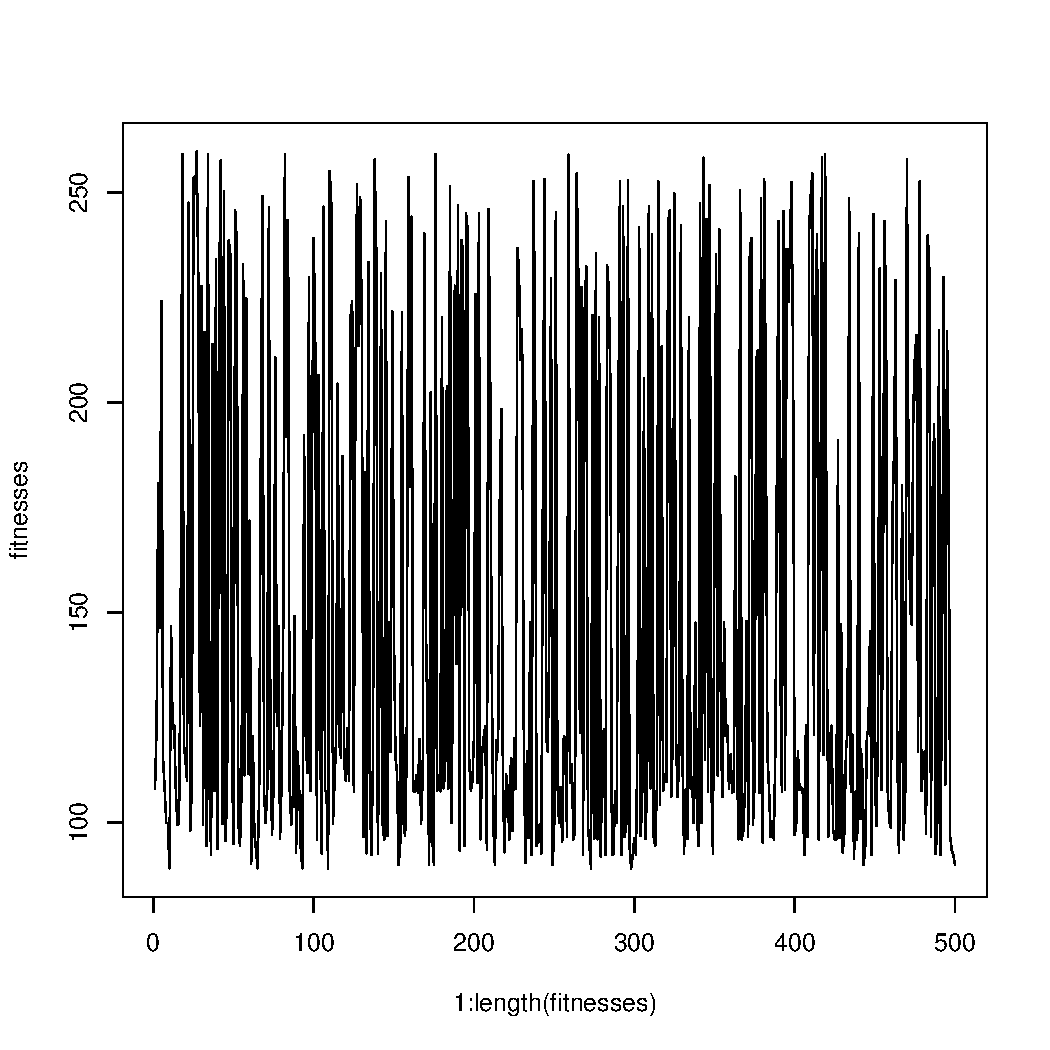
\includegraphics[width=60mm]{images/spherical.ss/ind_101.pdf}
		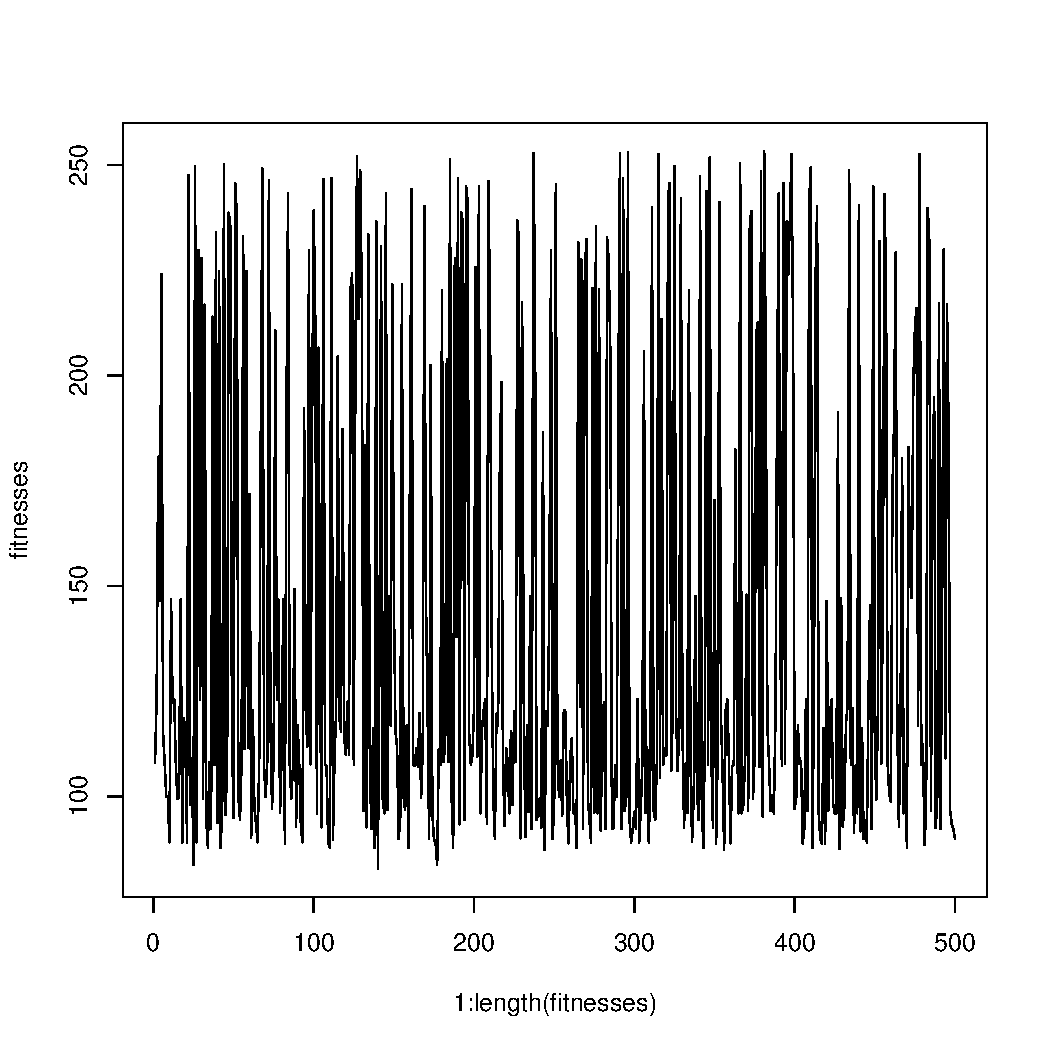
\includegraphics[width=60mm]{images/spherical.ss/ind_110.pdf}
		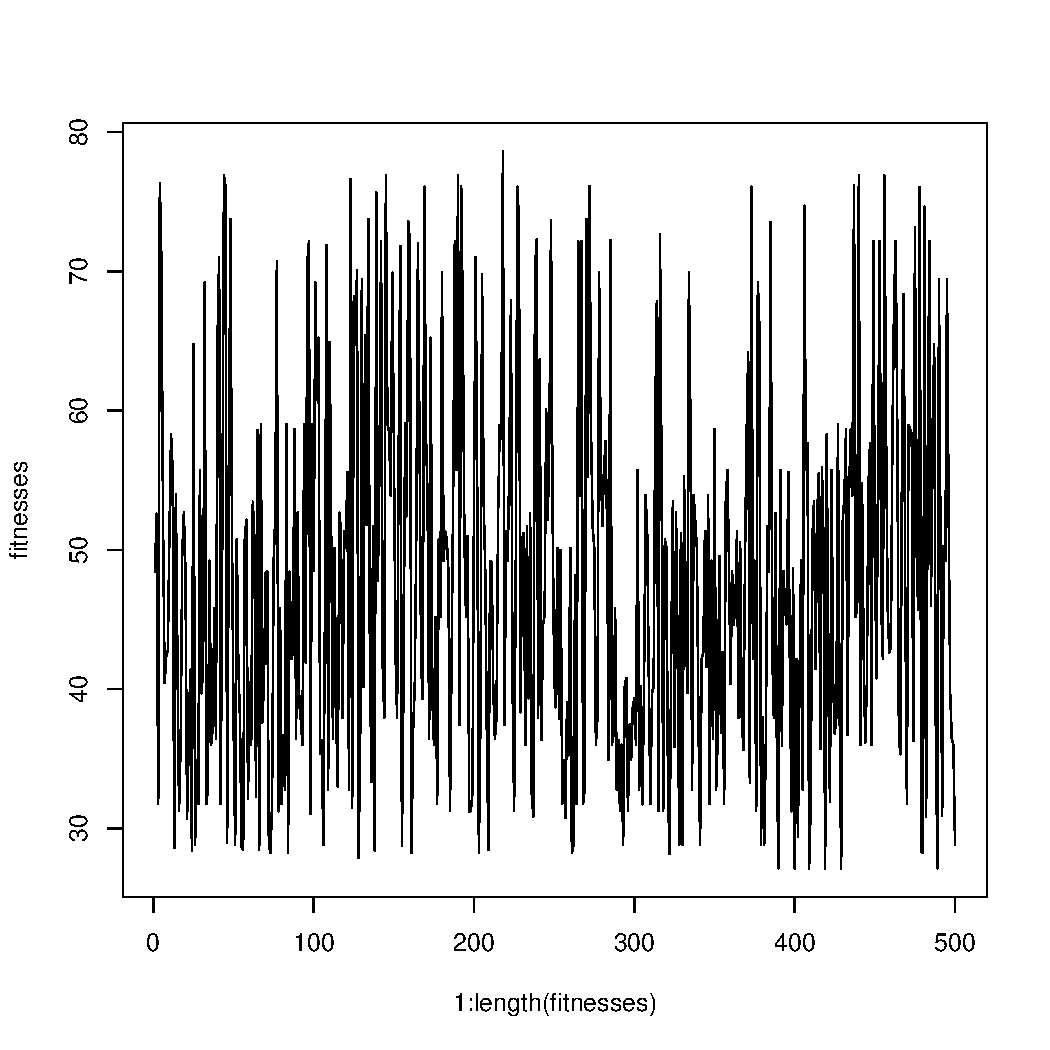
\includegraphics[width=60mm]{images/spherical.ss/ind_303.pdf}
		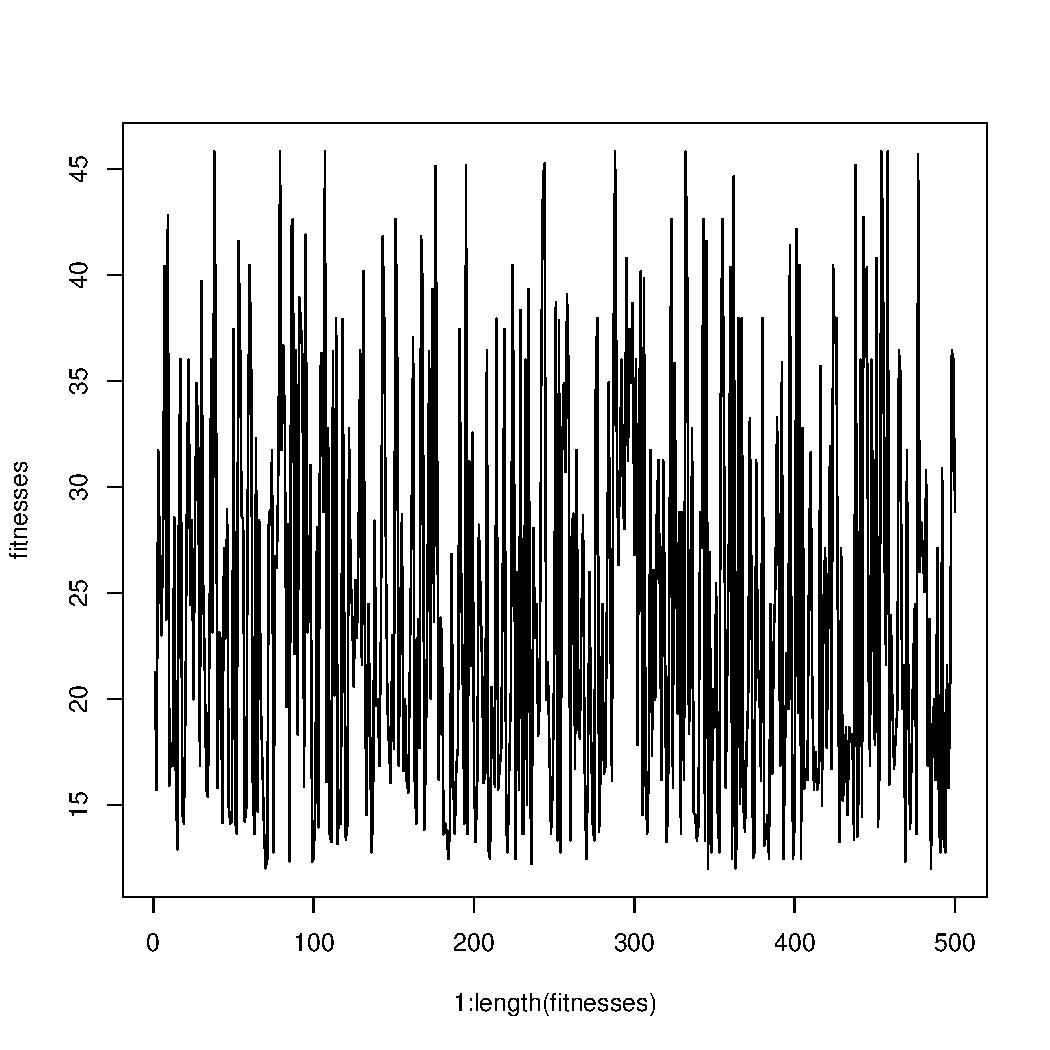
\includegraphics[width=60mm]{images/spherical.ss/ind_404.pdf}
               	\caption{Population fitnesses at 100, 110, 303, and 404 iterations, respectively}
                \label{spherical_ss_pop_fit}
        \end{center}
\end{figure}

The Spherical steady state GA converged to 0.00 at 7784 (8 minutes 52 seconds), and here was the lowest individual:
\scriptsize
\begin{lstlisting}
[1] "7784  - Avg fitness: 0.0001294 min: 1e-04 sd: 0.000644007088672571"
 [1] 0.00 0.00 0.00 0.00 0.00 0.00 0.00 0.01 0.00 0.00 0.00 0.00 0.00 0.00 0.00
[16] 0.00 0.00 0.00 0.00 0.00 0.00 0.00 0.00 0.00 0.00 0.00 0.00 0.00 0.00 0.00
[1] "Min fitnesses: 0"
[1] "Re-gen time: 0.0539999999999736"
\end{lstlisting}
\normalsize

%\pagebreak

\begin{figure}[!h]
        \begin{center}
		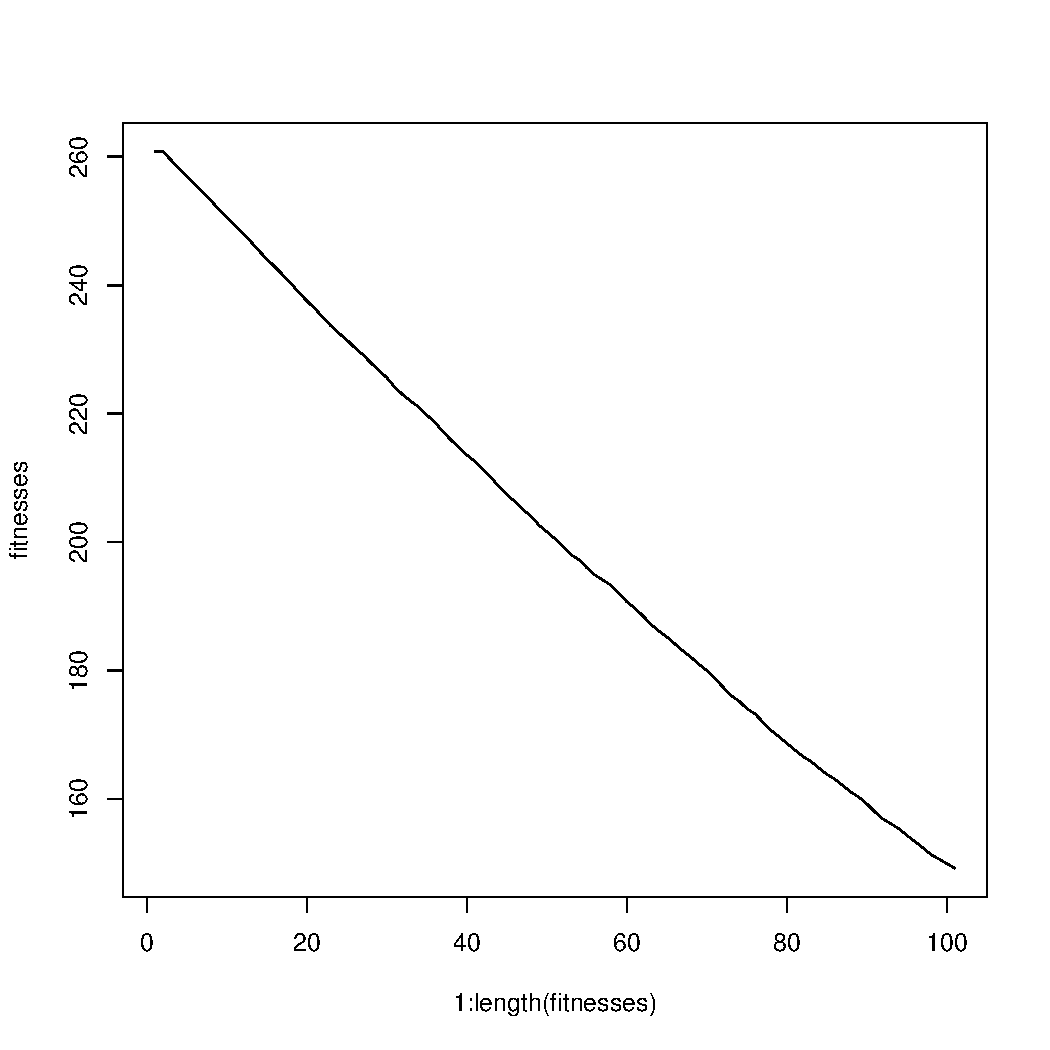
\includegraphics[width=60mm]{images/spherical.ss/avg_101.pdf}
		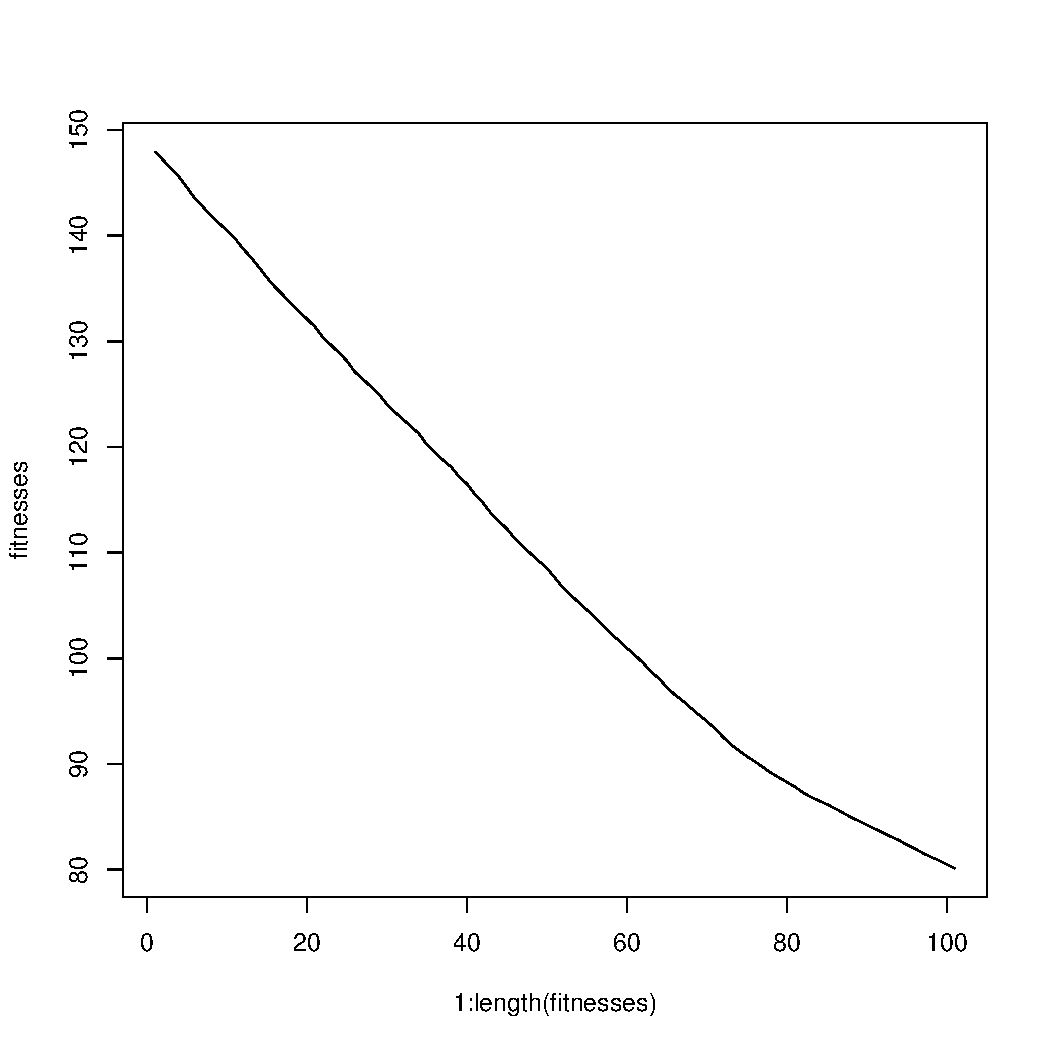
\includegraphics[width=60mm]{images/spherical.ss/avg_202.pdf}
		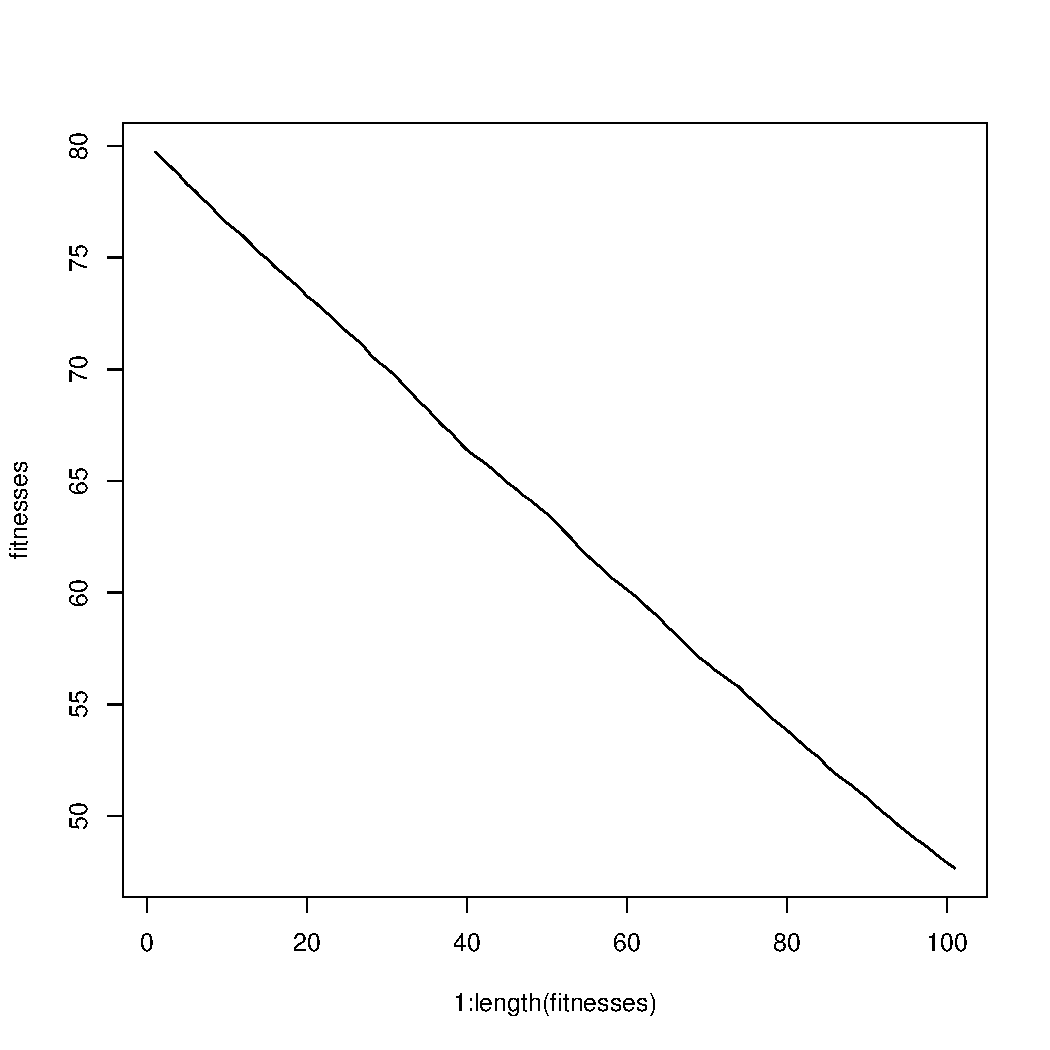
\includegraphics[width=60mm]{images/spherical.ss/avg_303.pdf}
		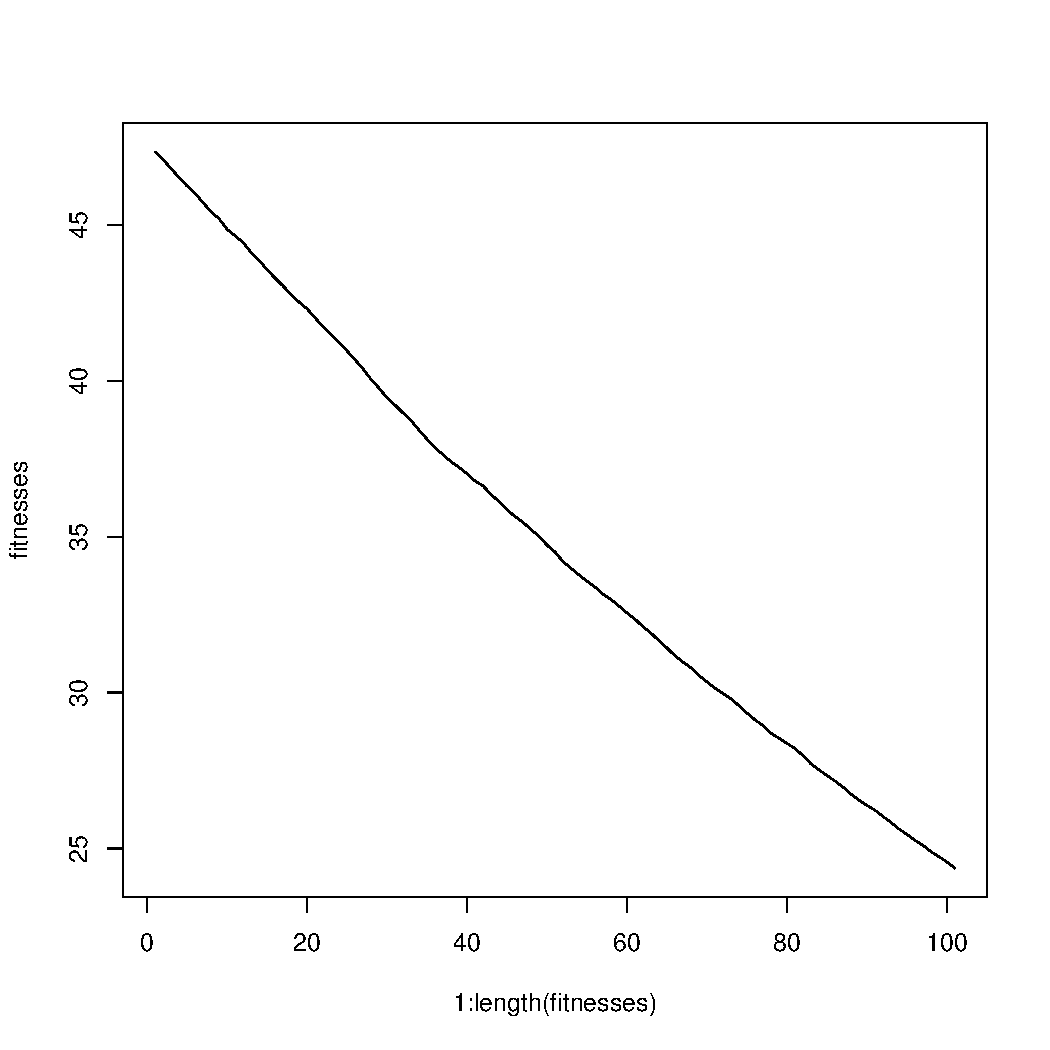
\includegraphics[width=60mm]{images/spherical.ss/avg_404.pdf}
               	\caption{Average population fitnesses at 100, 202, 303, and 404 iterations, respectively, at 100 iteration wide snapshots}
                \label{spherical_ss_avg_pop_fit}
        \end{center}
\end{figure}


\pagebreak

\section{Rosenbrock}
\begin{figure}[!h]
        \begin{center}
		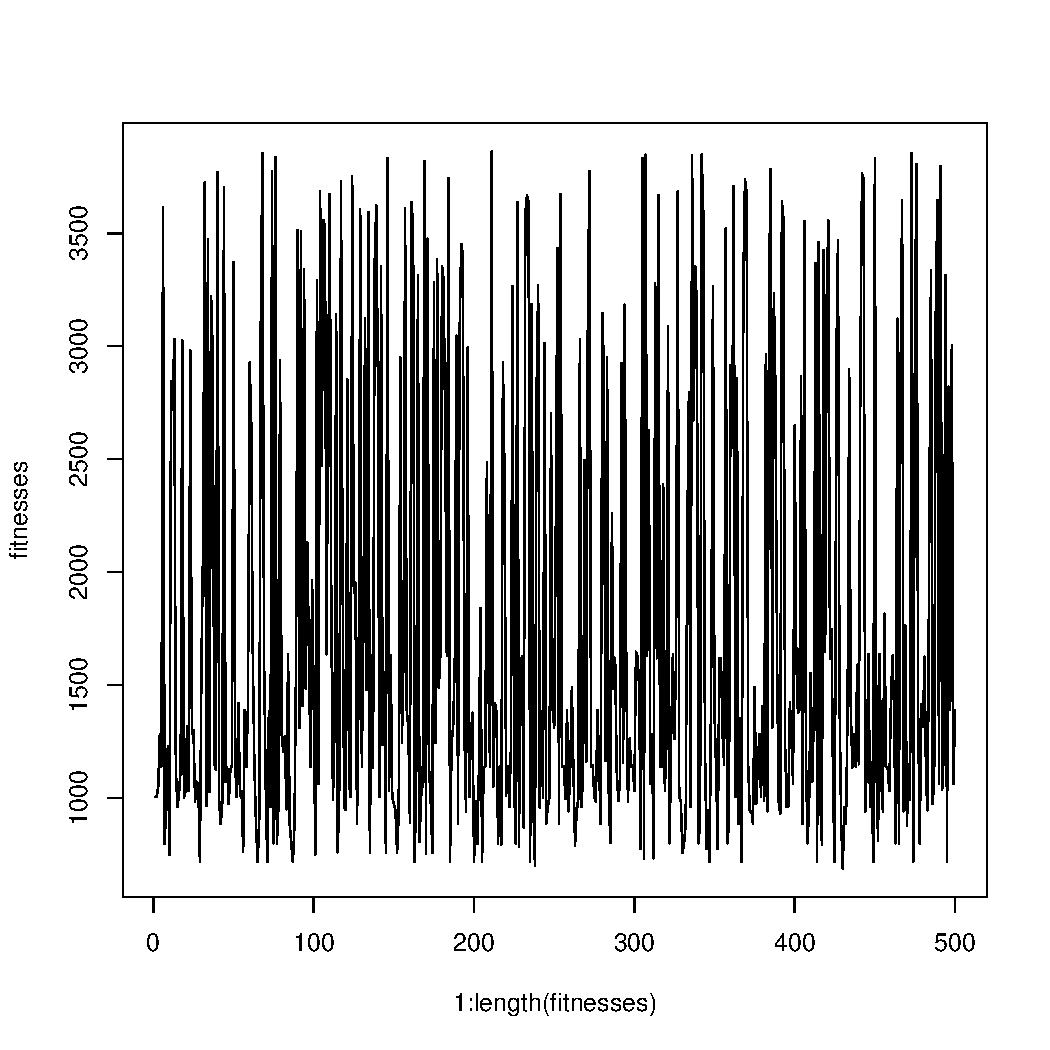
\includegraphics[width=60mm]{images/rosenbrock.ss/ind_110.pdf}
		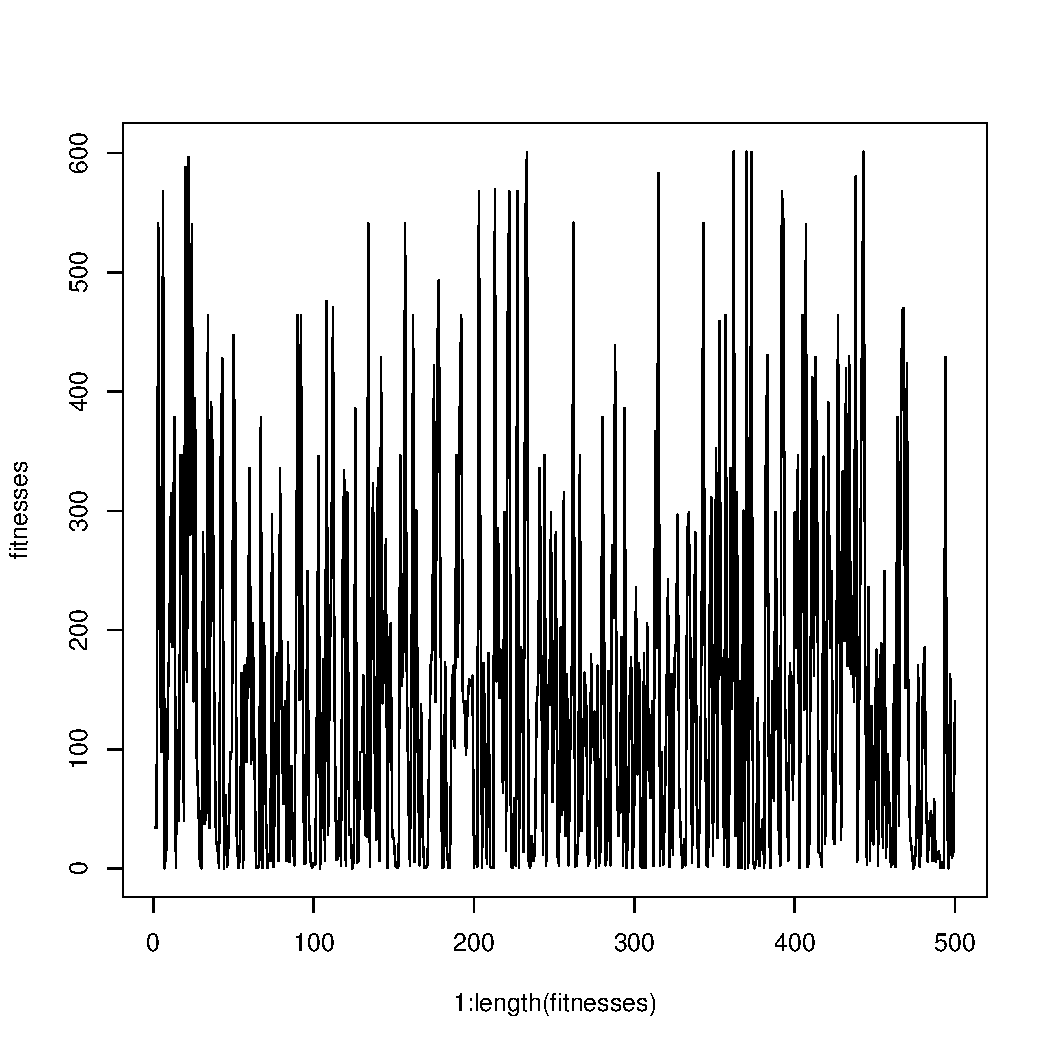
\includegraphics[width=60mm]{images/rosenbrock.ss/ind_303.pdf}
		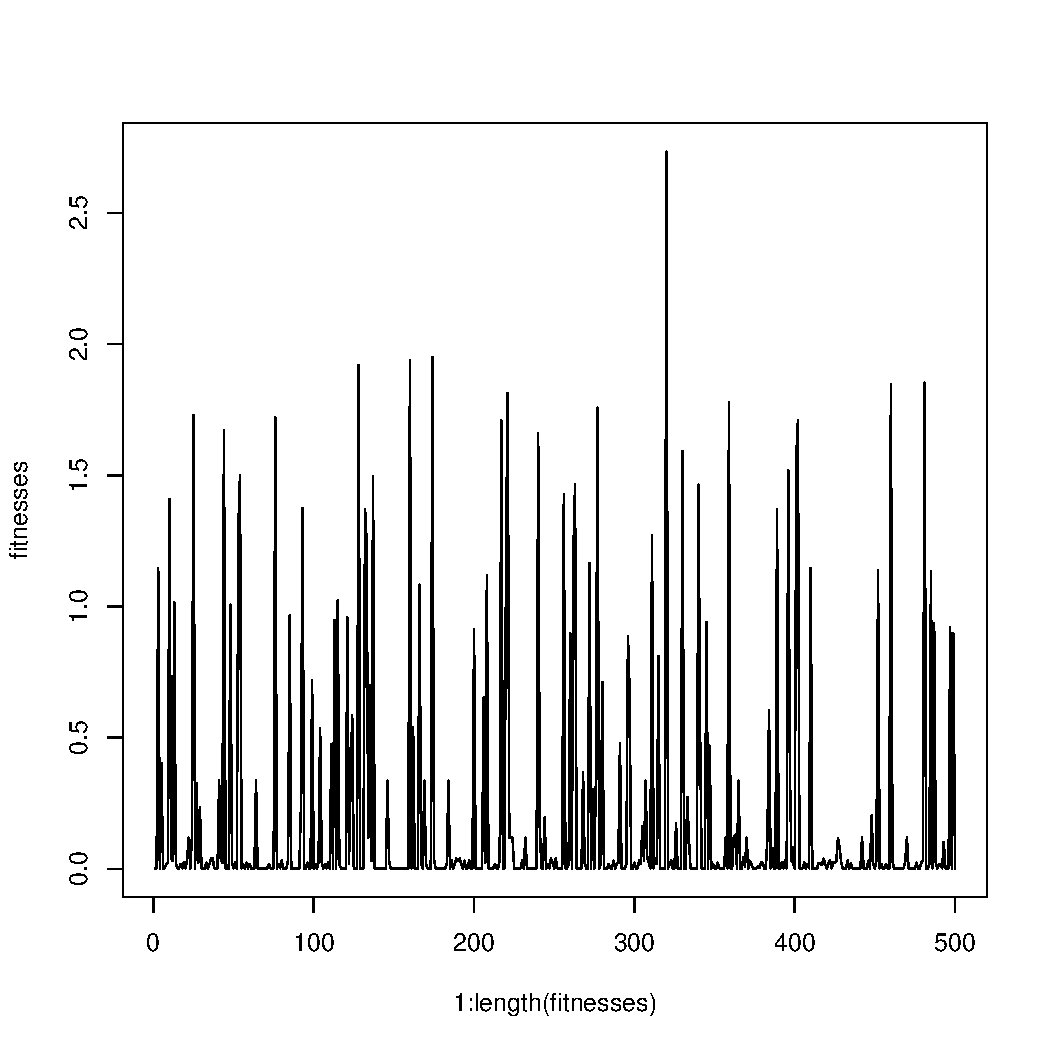
\includegraphics[width=60mm]{images/rosenbrock.ss/ind_707.pdf}
		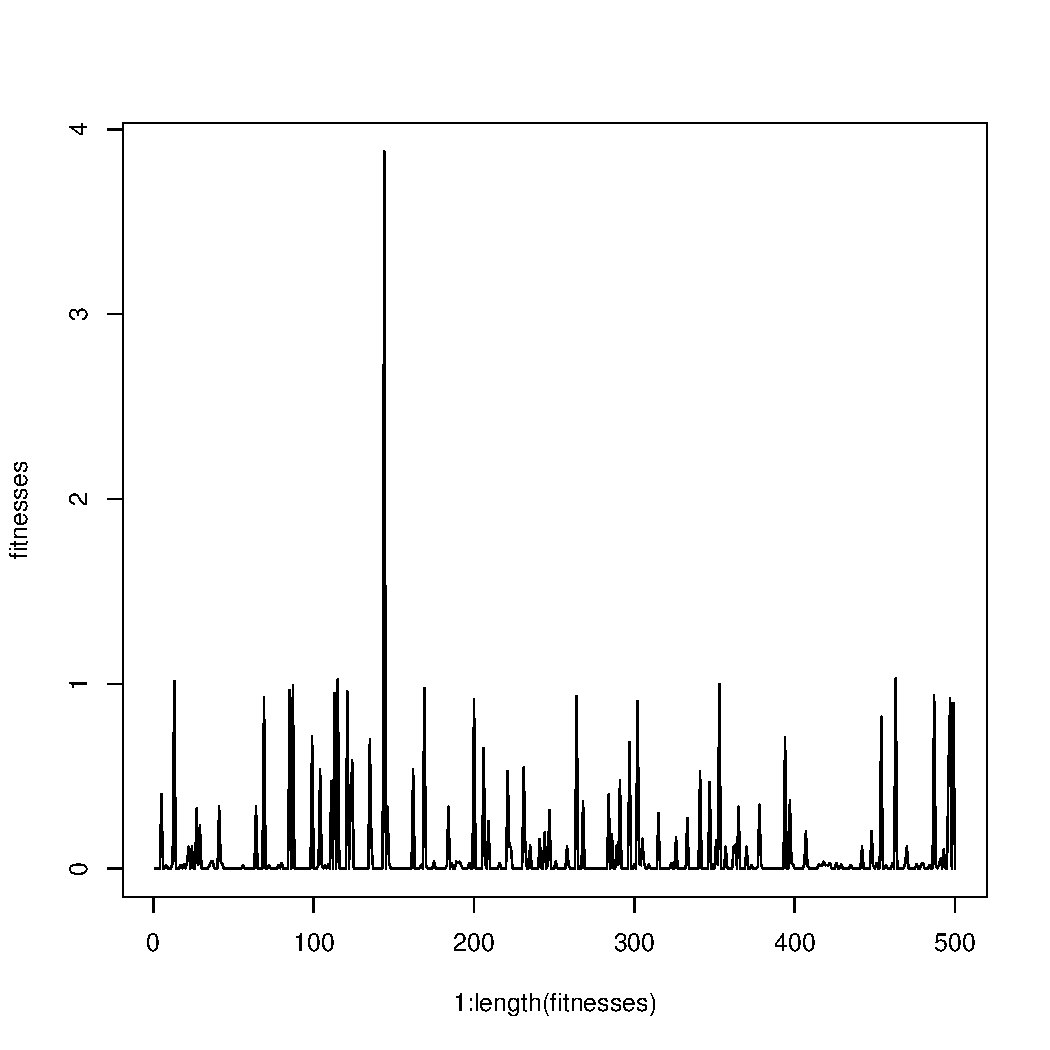
\includegraphics[width=60mm]{images/rosenbrock.ss/ind_808.pdf}
               	\caption{Population fitnesses at 110, 303, 707, and 808 iterations, respectively, to highlight slow steady state crossovers}
                \label{rosenbrock_ss_pop_fit}
        \end{center}
\end{figure}

Due to the increased precision in the domain, this function required a change Figure \ref{creep_mutation} $S$ value from $.10 $ to $.01$.  The Rosenbrock steady state GA never converged to 0.00, and at 10,000 generations (34 minutes 44 seconds), the lowest individual was:
\scriptsize
\begin{lstlisting}
[1] "10000  - Avg fitness: 0.00937186799996092 min: 0.00172399999996076 sd: 0.169202076655399"
 [1]  0.229  0.520  0.812  0.320 -0.013  0.693  1.030 -0.271  0.711 -0.109
[11]  0.446  0.224  0.392  0.258  0.733  1.142 -0.427 -0.442  0.460  0.954
[21]  0.204  0.847  0.756 -0.404  0.298  0.325 -0.531  0.450  0.273 -0.562
[1] "Min fitnesses: 0.00172399999996076"
[1] "Re-gen time: 0.210000000000036"
\end{lstlisting}
\normalsize

\pagebreak

\begin{figure}[!h]
        \begin{center}
		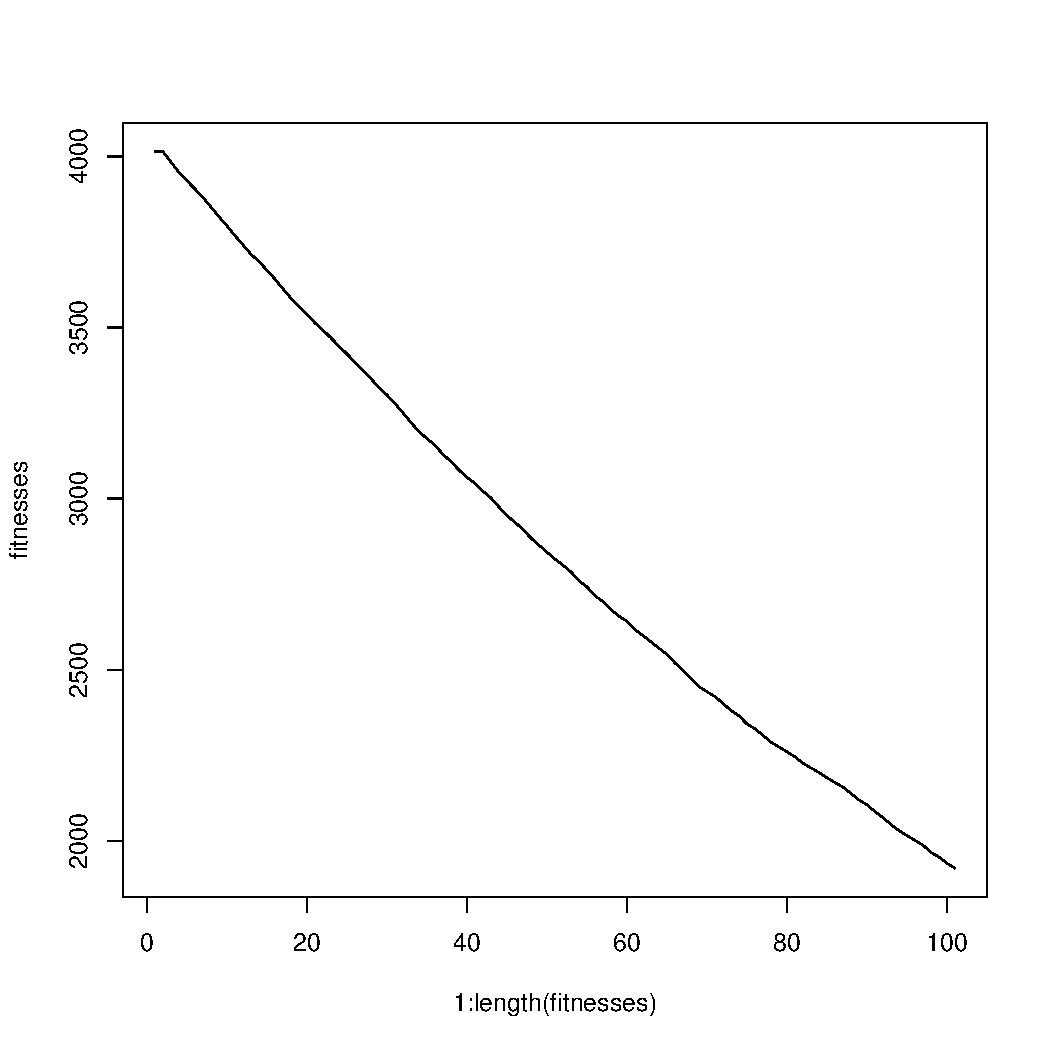
\includegraphics[width=60mm]{images/rosenbrock.ss/avg_101.pdf}
		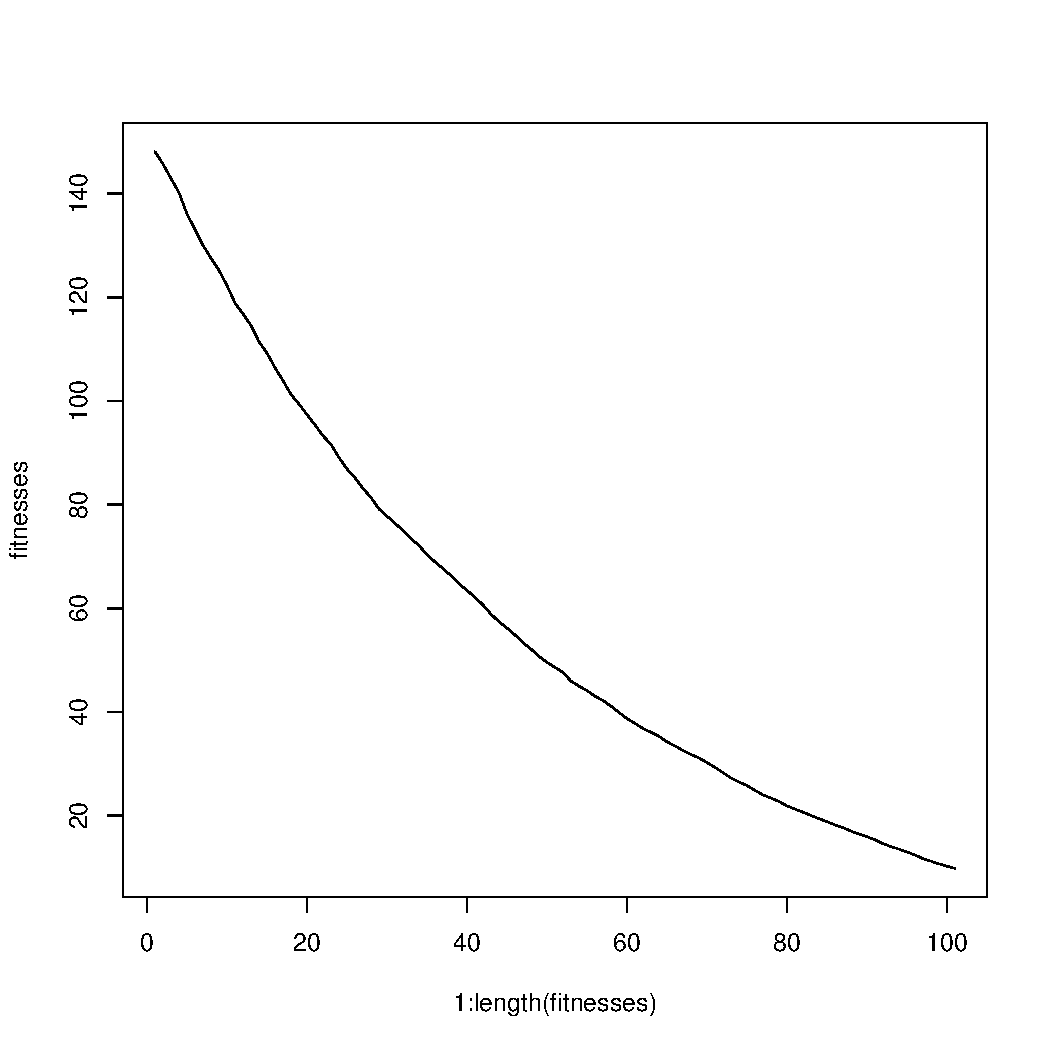
\includegraphics[width=60mm]{images/rosenbrock.ss/avg_404.pdf}
		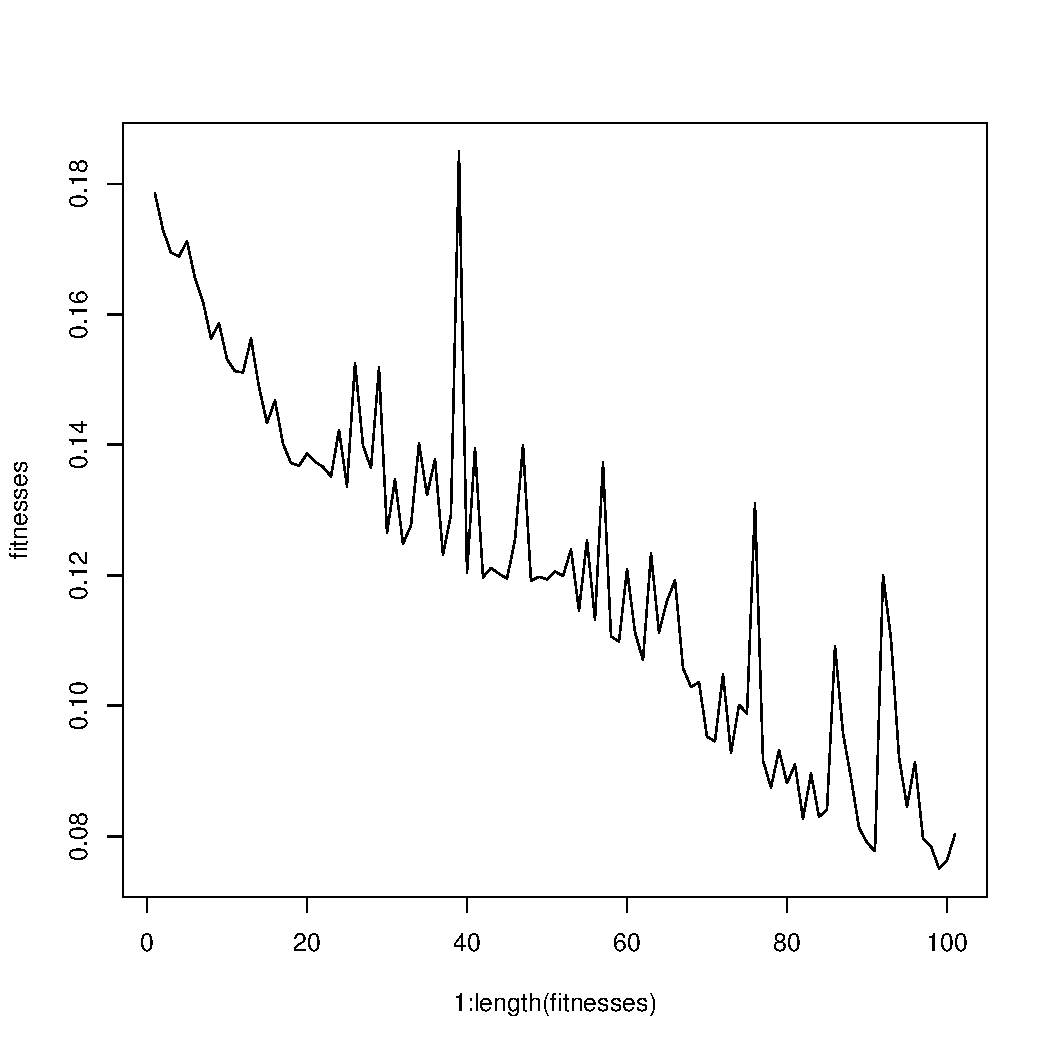
\includegraphics[width=60mm]{images/rosenbrock.ss/avg_808.pdf}
		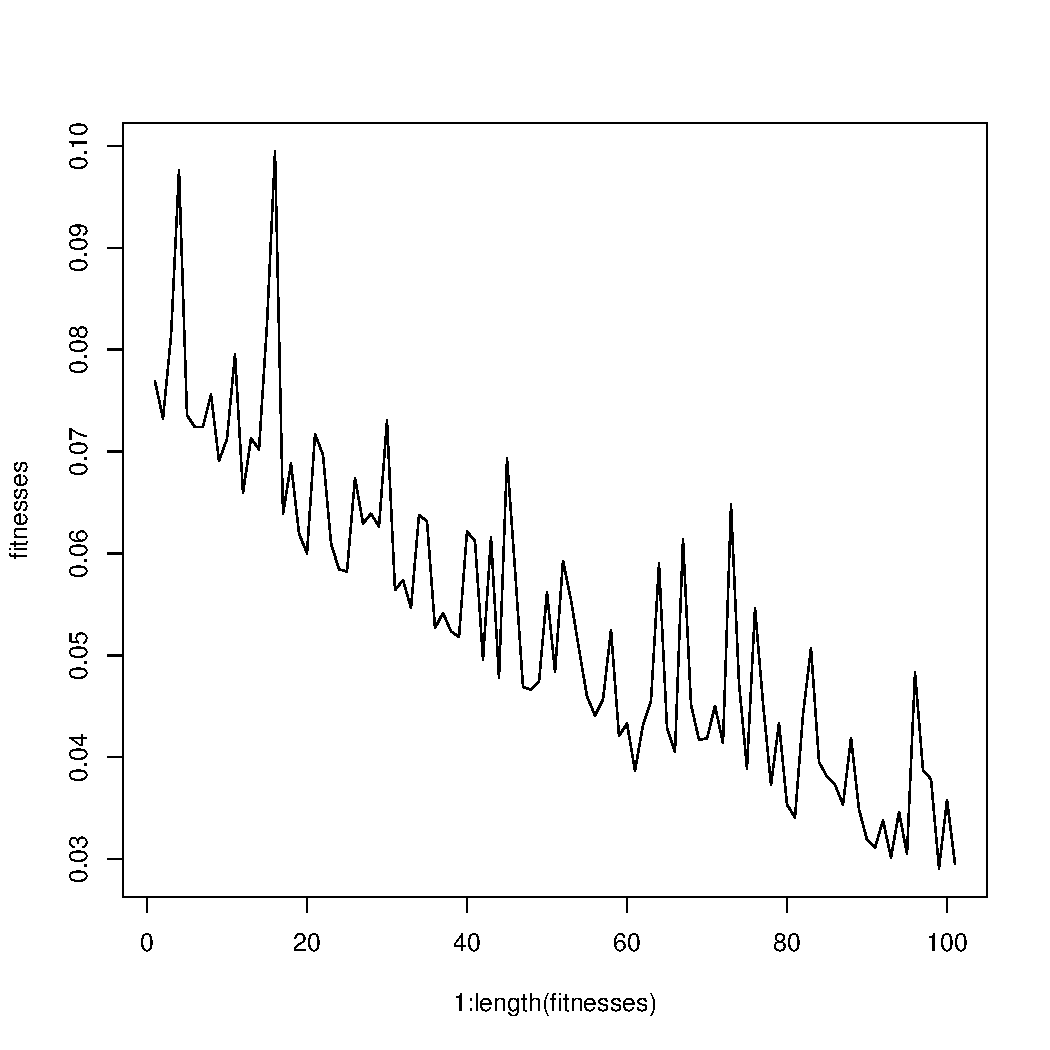
\includegraphics[width=60mm]{images/rosenbrock.ss/avg_909.pdf}
               	\caption{Average population fitnesses at 100, 404, 808, and 909 iterations, respectively, at 100 iteration wide snapshots}
                \label{rosenbrock_ss_avg_pop_fit}
        \end{center}
\end{figure}


\pagebreak

\section{Rastrigin}
\begin{figure}[!h]
        \begin{center}
		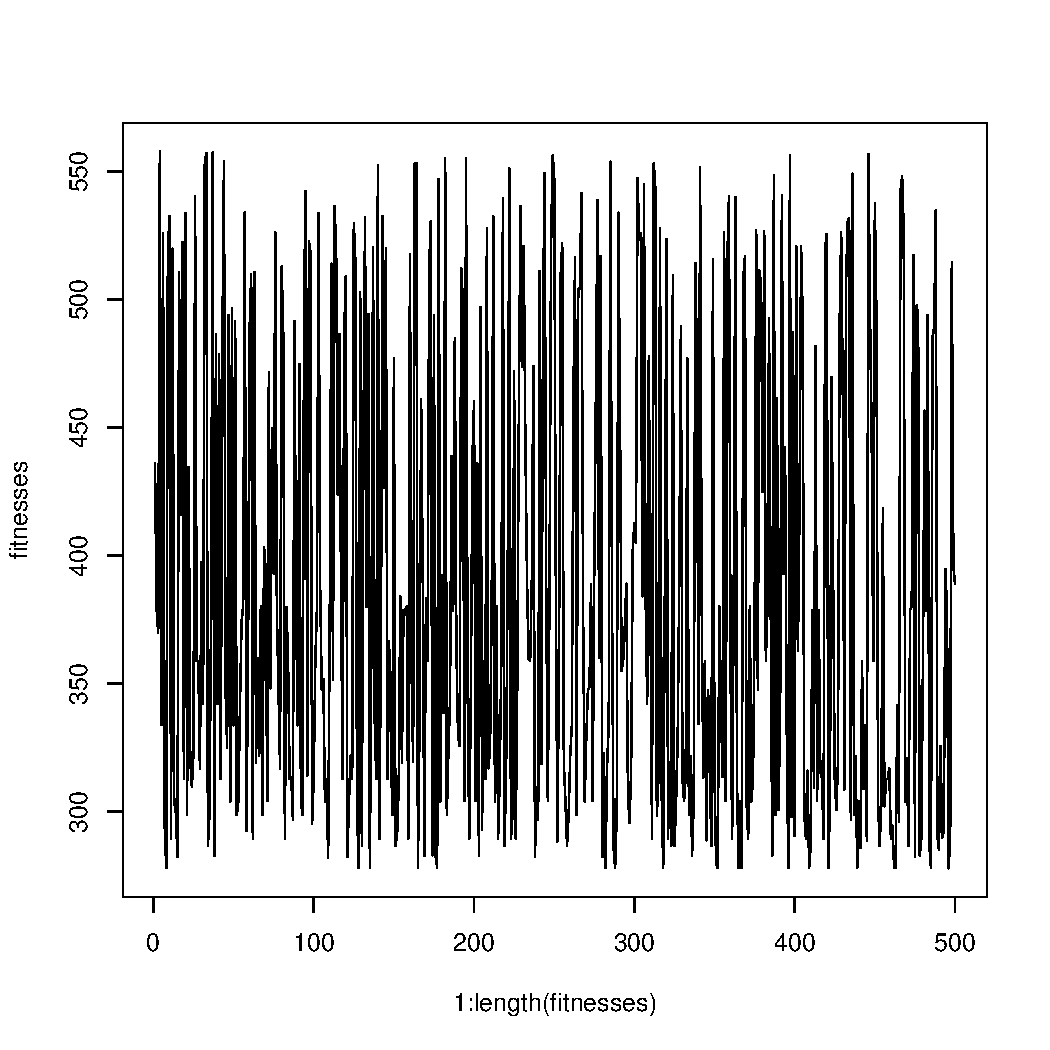
\includegraphics[width=60mm]{images/rastrigin.ss/ind_101.pdf}
		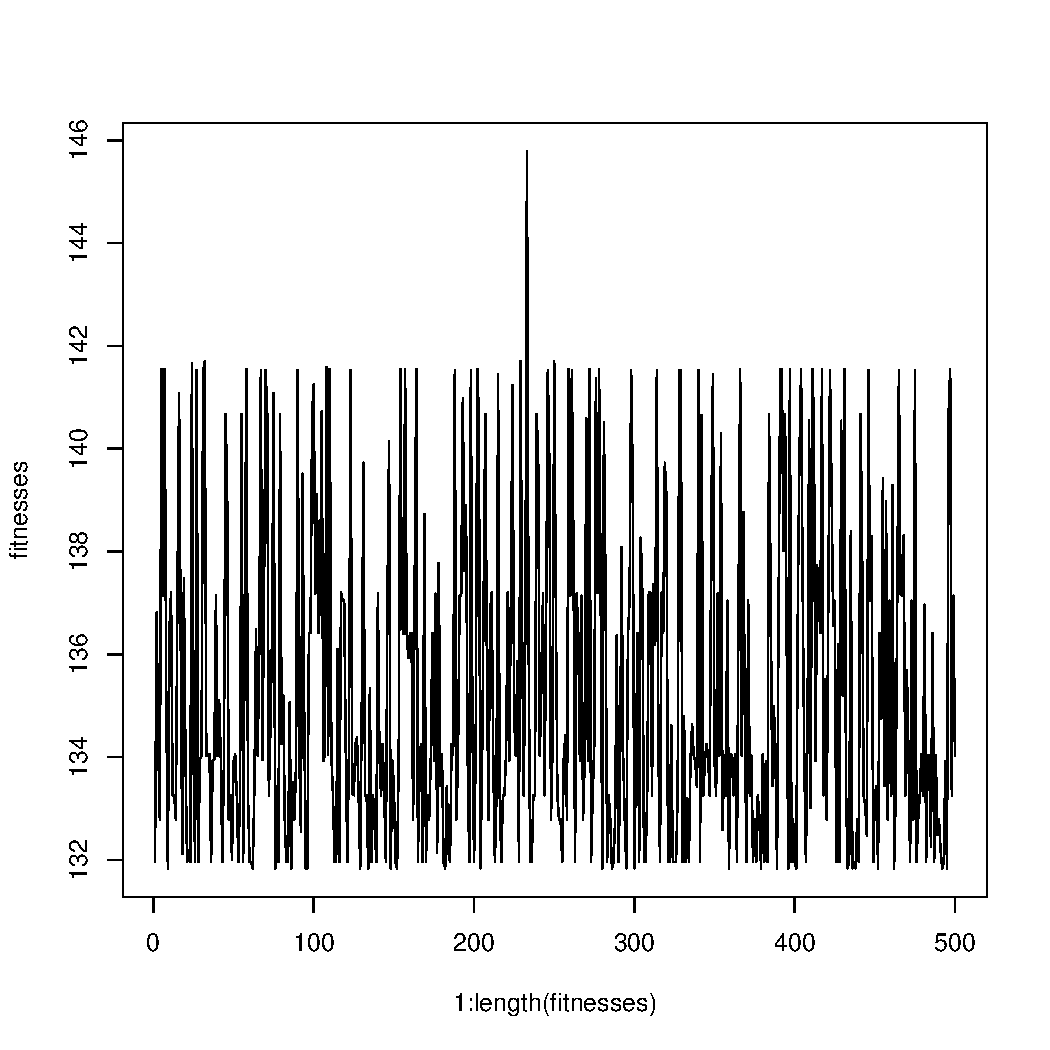
\includegraphics[width=60mm]{images/rastrigin.ss/ind_1212.pdf}
		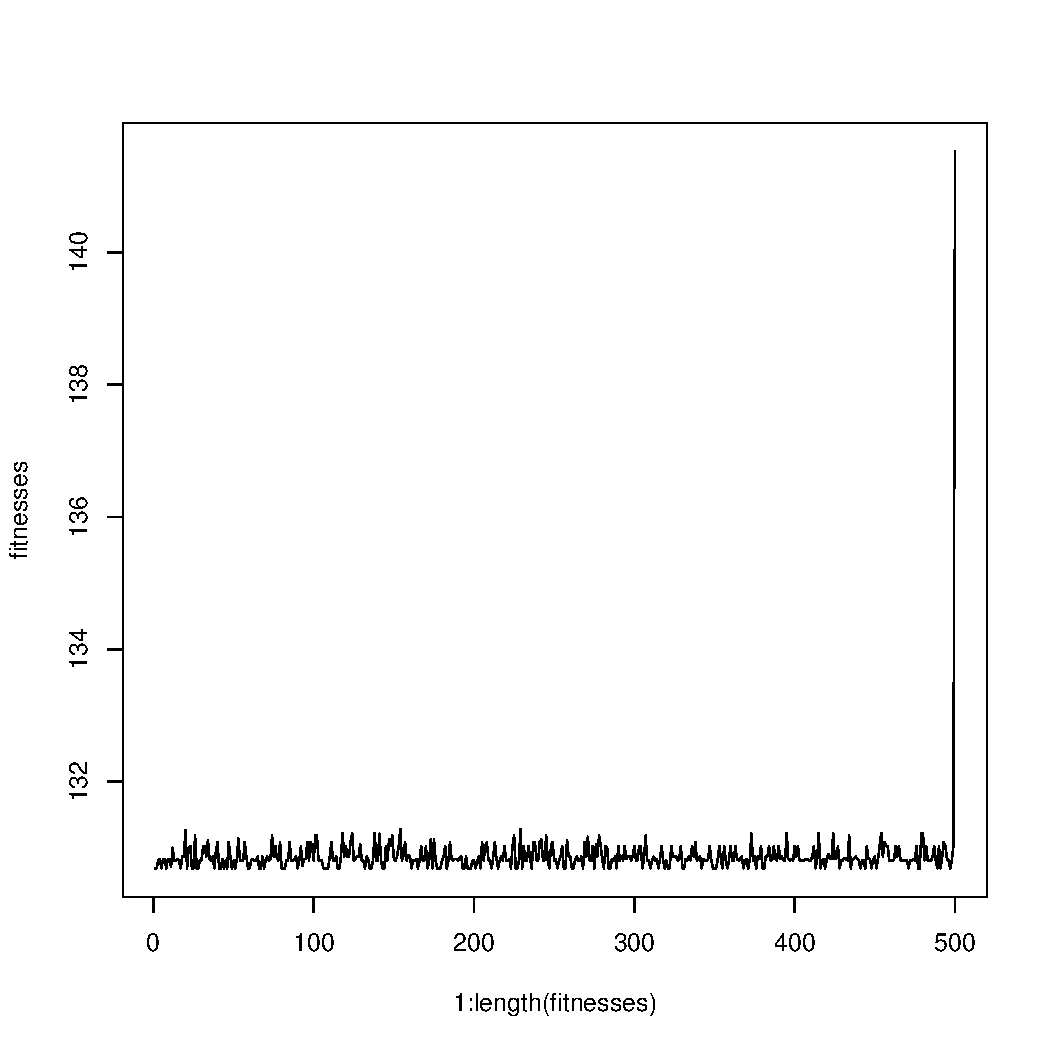
\includegraphics[width=60mm]{images/rastrigin.ss/ind_2020.pdf}
		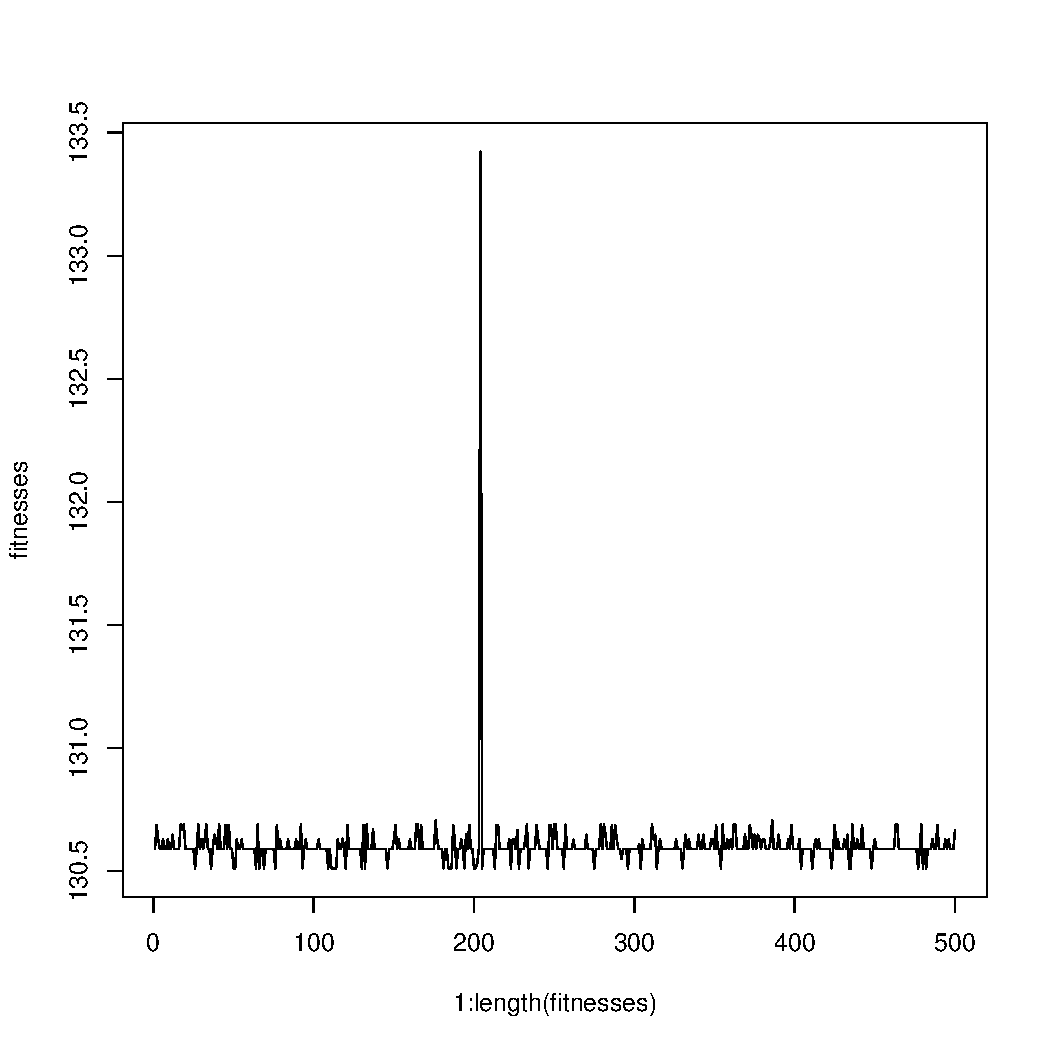
\includegraphics[width=60mm]{images/rastrigin.ss/ind_2828.pdf}
               	\caption{Population fitnesses at 100, 1212, 2020, and 2828 iterations, respectively}
                \label{rastrigin_ss_pop_fit}
        \end{center}
\end{figure}

The Rastrigin steady state GA never converged to 0.00, and at 10,000 generations (32 minutes 21 seconds), the lowest individual was:
\scriptsize
\begin{lstlisting}
[1] "10000  - Avg fitness: 130.416021401637 min: 130.410678209187 sd: 0.11947741535045"
 [1] -0.99  1.99  2.98  2.98 -1.99  0.00  1.99 -1.99 -1.99 -1.99 -2.98  0.00
[13] -0.99  2.98 -1.99  0.99  1.99 -1.99  2.98 -2.98  1.99  0.99 -0.99 -1.99
[25]  1.99  0.99 -1.99 -0.99  2.98  2.98
[1] "Min fitnesses: 130.410678209187"
[1] "Re-gen time: 0.200000000000273"
\end{lstlisting}
\normalsize

\pagebreak

\begin{figure}[!h]
        \begin{center}
		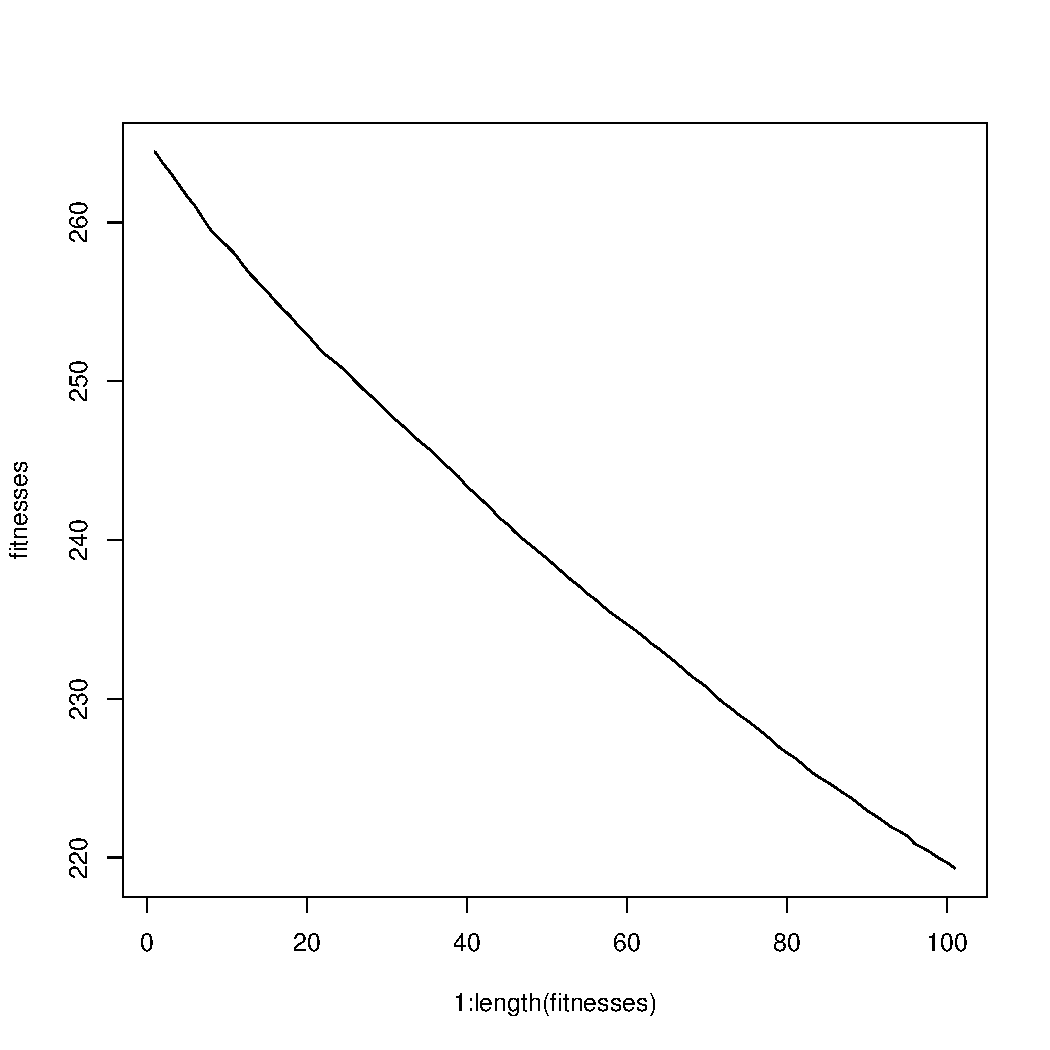
\includegraphics[width=60mm]{images/rastrigin.ss/avg_303.pdf}
		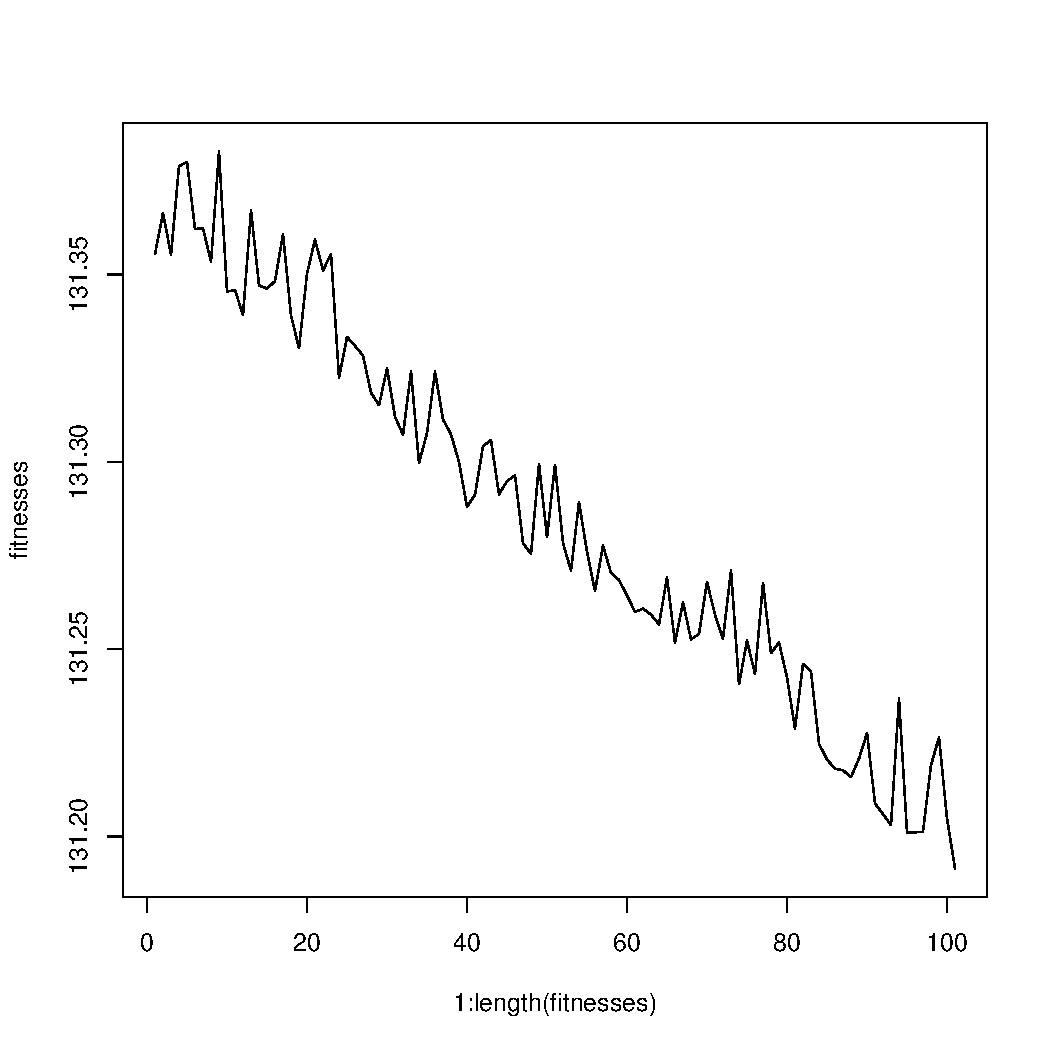
\includegraphics[width=60mm]{images/rastrigin.ss/avg_1717.pdf}
		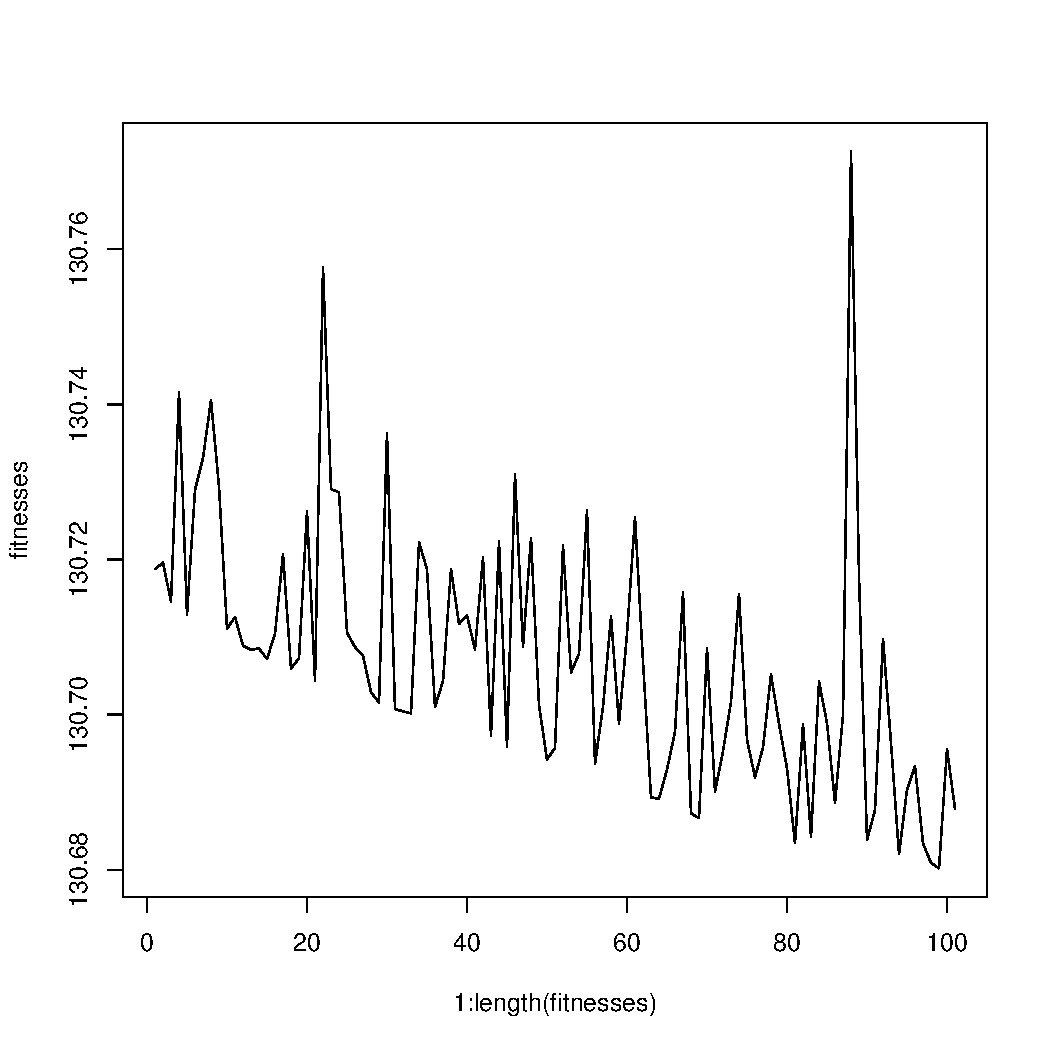
\includegraphics[width=60mm]{images/rastrigin.ss/avg_2424.pdf}
		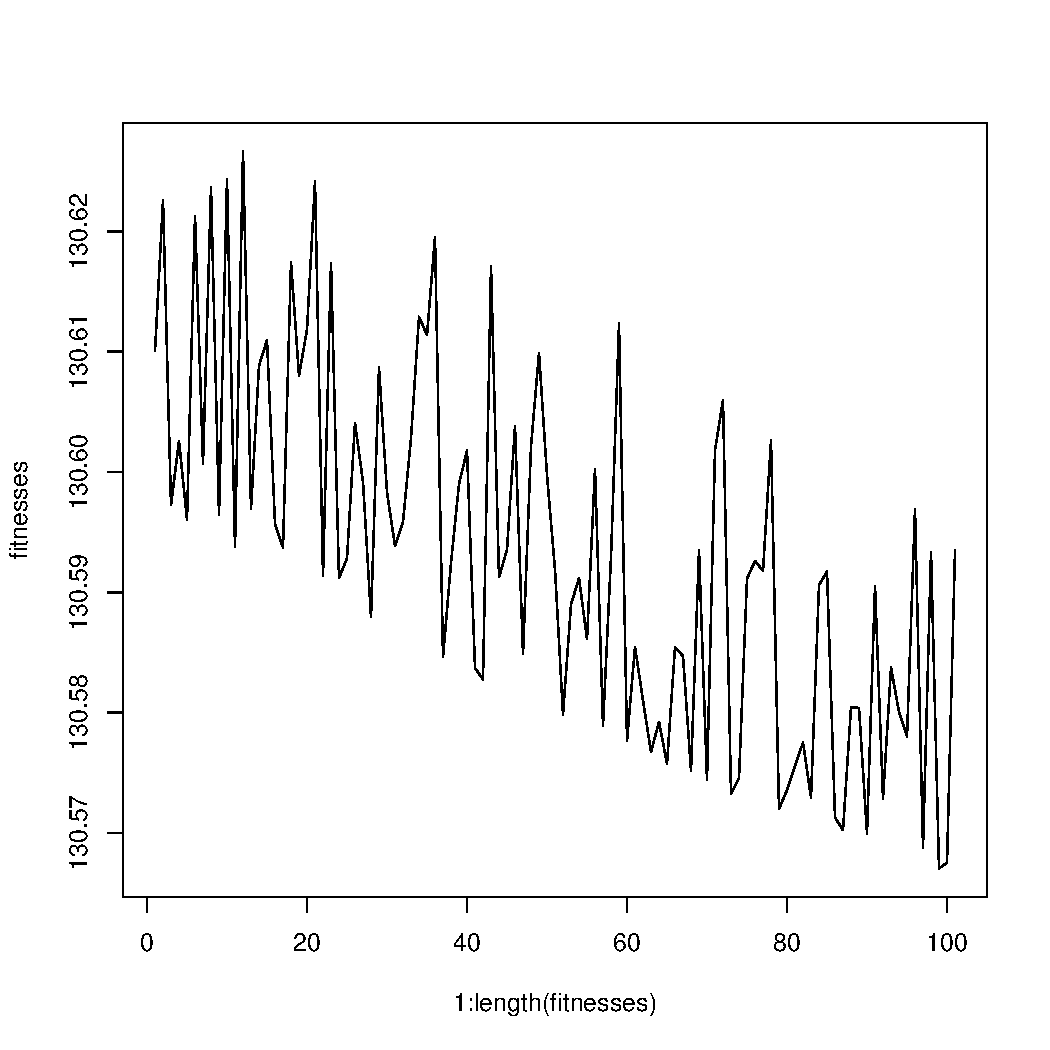
\includegraphics[width=60mm]{images/rastrigin.ss/avg_2929.pdf}
               	\caption{Average population fitnesses at 303, 1717, 2424, and 2929 iterations, respectively, at 100 iteration wide snapshots}
                \label{rastrigin_ss_avg_pop_fit}
        \end{center}
\end{figure}


\pagebreak

\section{Schwefel}
\begin{figure}[!h]
        \begin{center}
		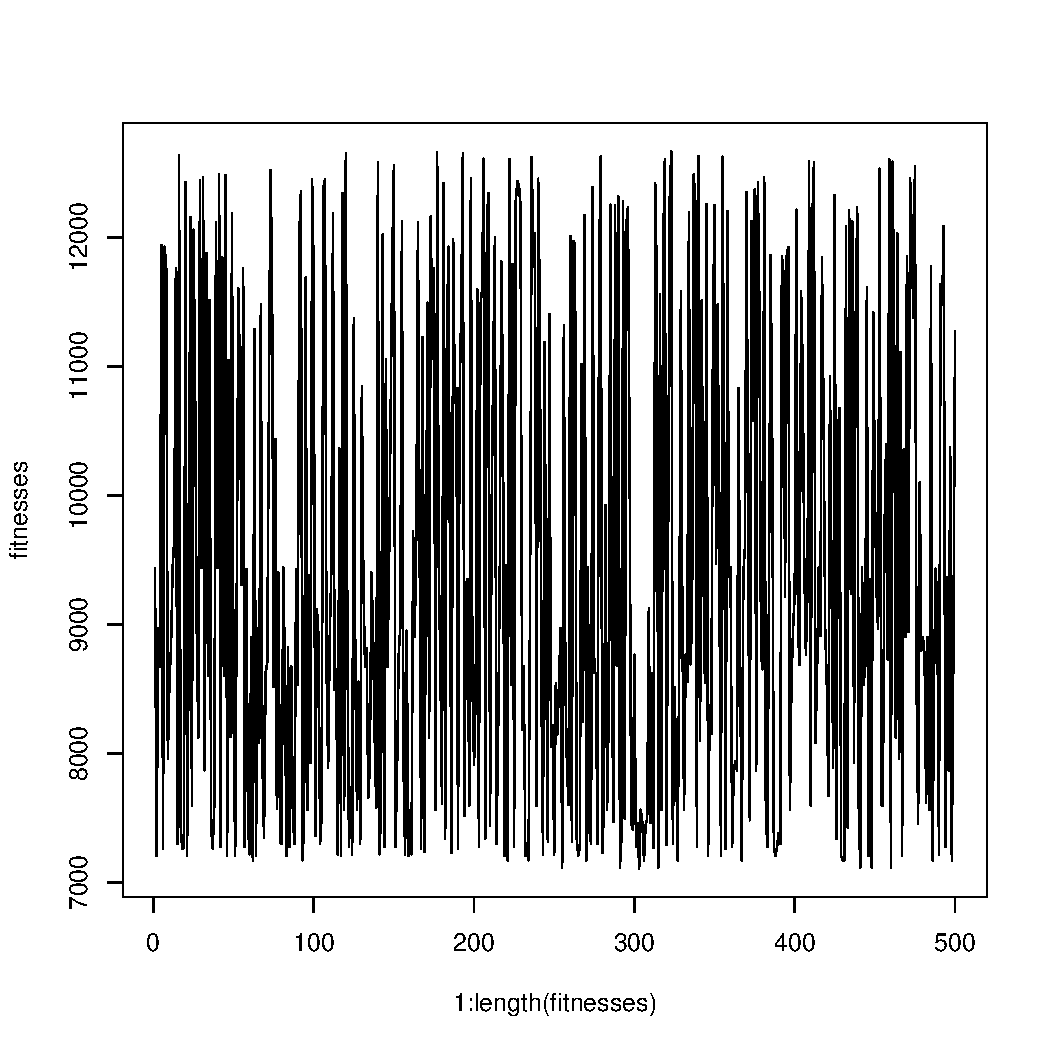
\includegraphics[width=60mm]{images/schwefel.ss/ind_101.pdf}
		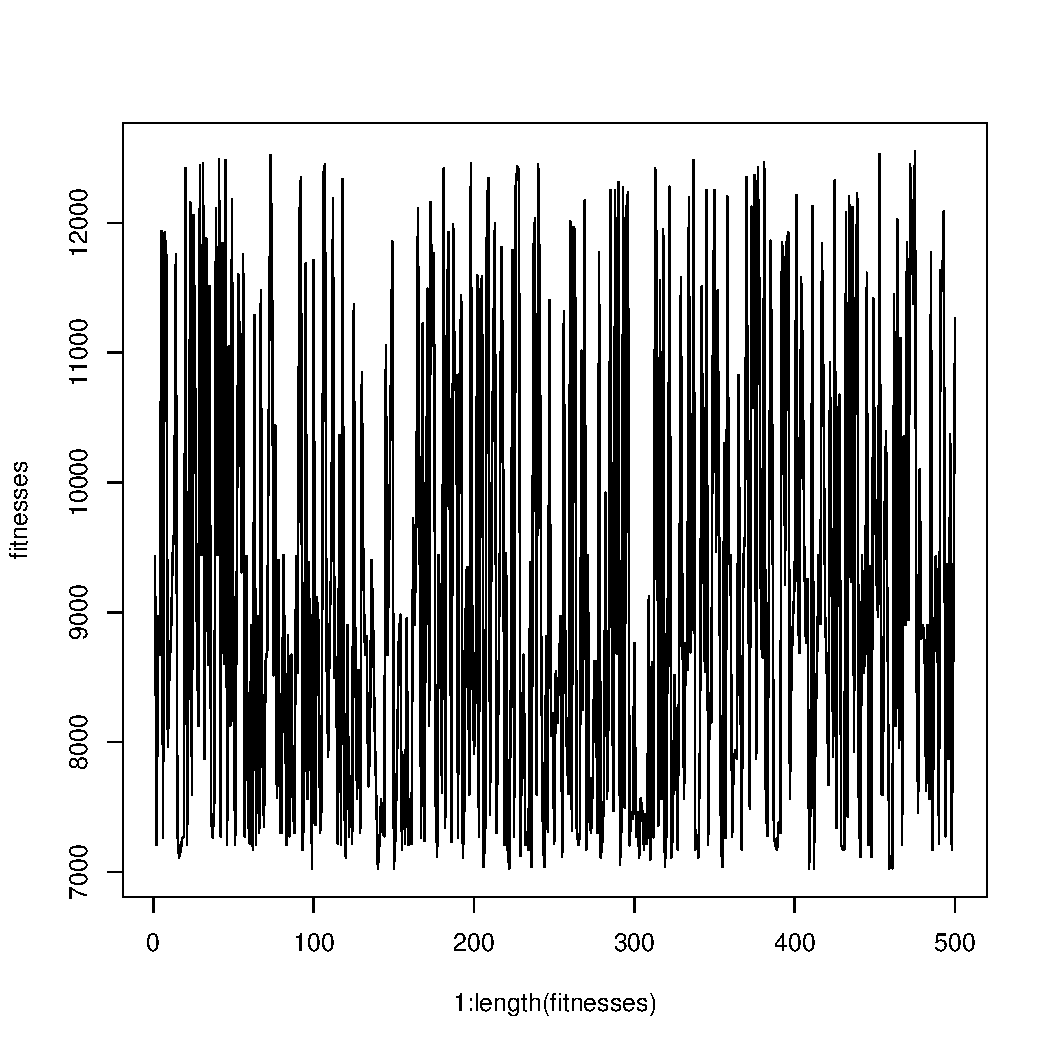
\includegraphics[width=60mm]{images/schwefel.ss/ind_110.pdf}
		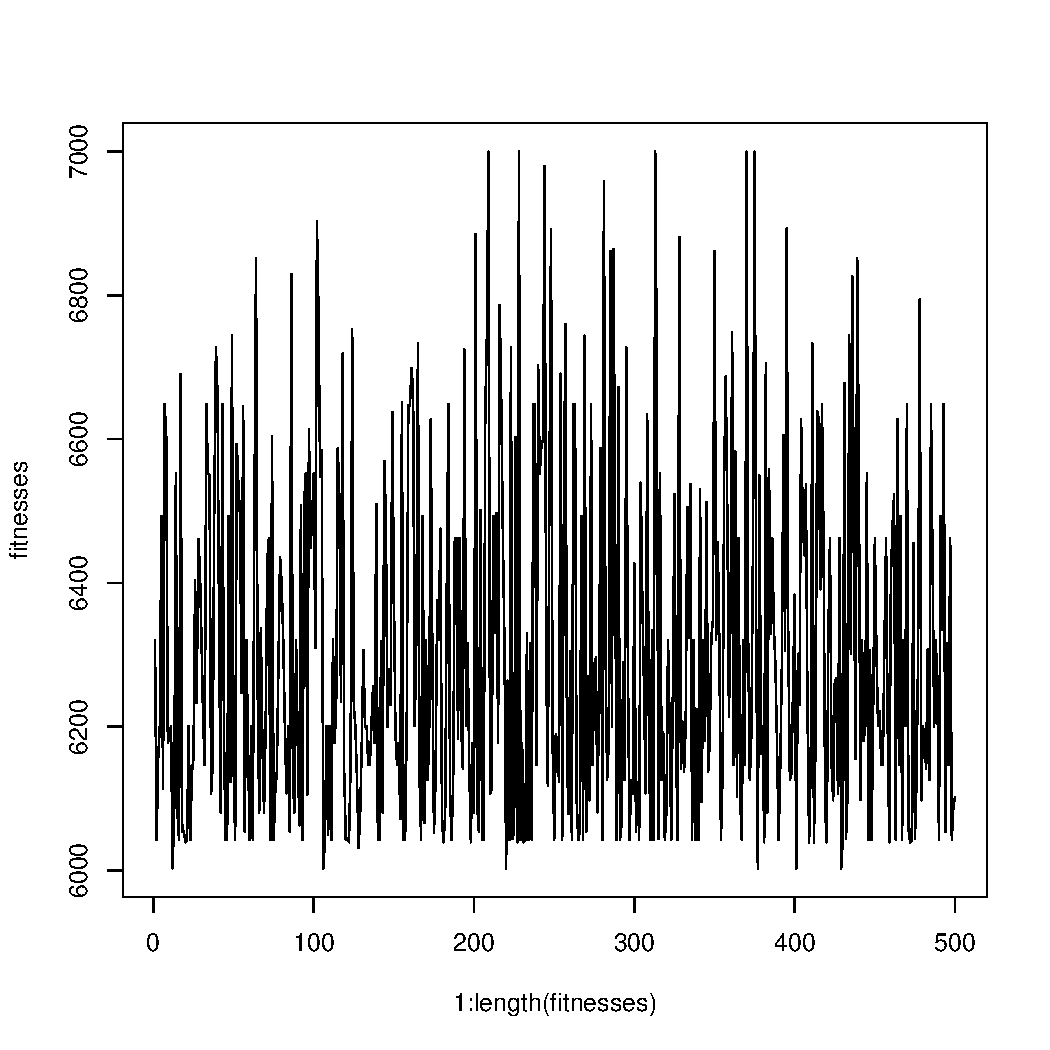
\includegraphics[width=60mm]{images/schwefel.ss/ind_303.pdf}
		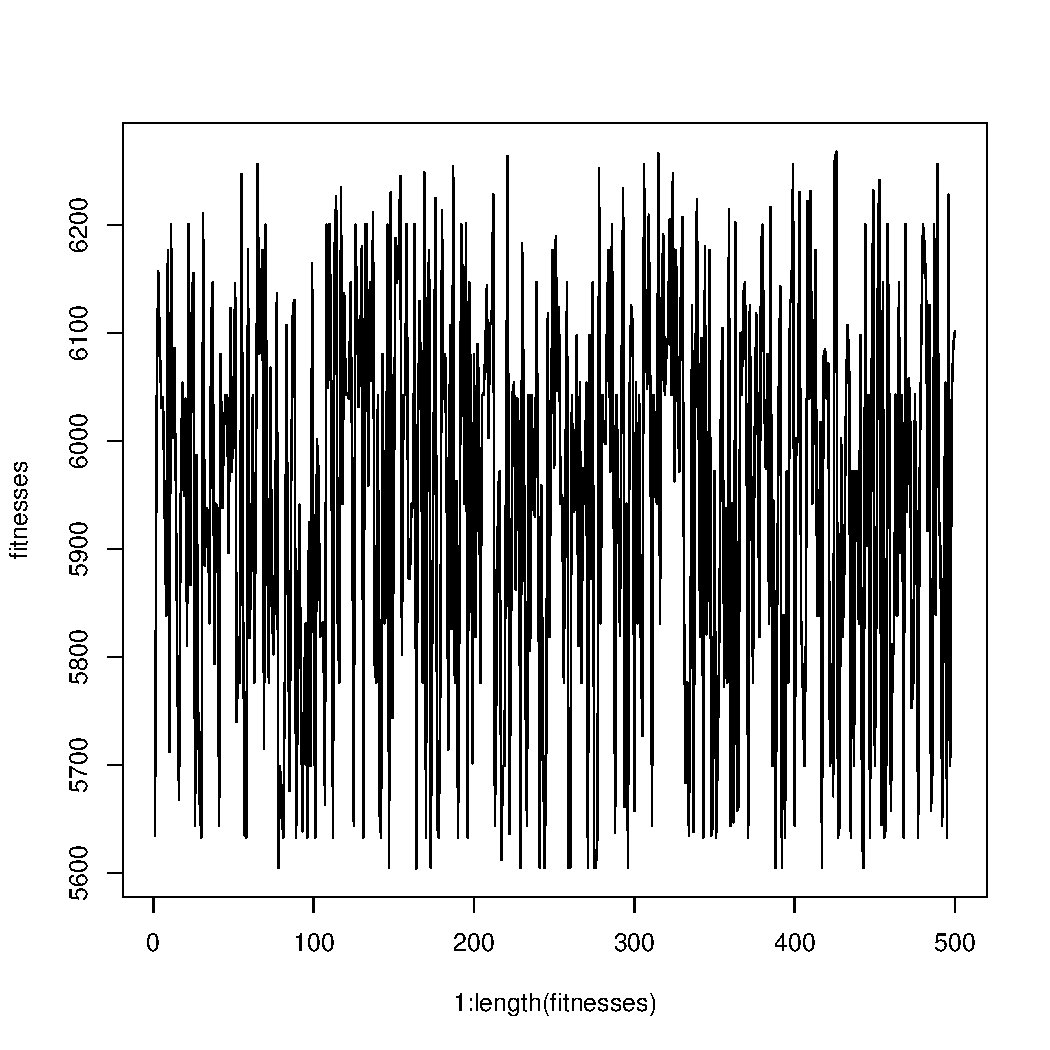
\includegraphics[width=60mm]{images/schwefel.ss/ind_404.pdf}
               	\caption{Population fitnesses at 100, 110, 303, and 404 iterations, respectively}
                \label{schwefel_ss_pop_fit}
        \end{center}
\end{figure}

The Schwefel steady state GA never converged to its 0, and at 10,000 generations (31 minutes 40 seconds), the lowest individual was:
\scriptsize
\begin{lstlisting}
[1] "10000  - Avg fitness: 4544.40077437804 min: 4544.34247297431 sd: 1.14760295955693"
 [1]  302.49  124.83  -65.76  302.52 -204.21  302.58 -204.17  302.55  124.69
[10] -420.95  302.61  494.35  124.92  302.52 -420.94 -420.98  302.48  302.53
[19] -421.02 -420.87 -203.66 -421.48  302.53  124.89 -203.71 -203.74  302.50
[28] -203.63 -203.84 -420.95
[1] "Min fitnesses: 4544.34247297431"
[1] "Re-gen time: 0.176000000000158"

\end{lstlisting}
\normalsize

\pagebreak

\begin{figure}[!h]
        \begin{center}
		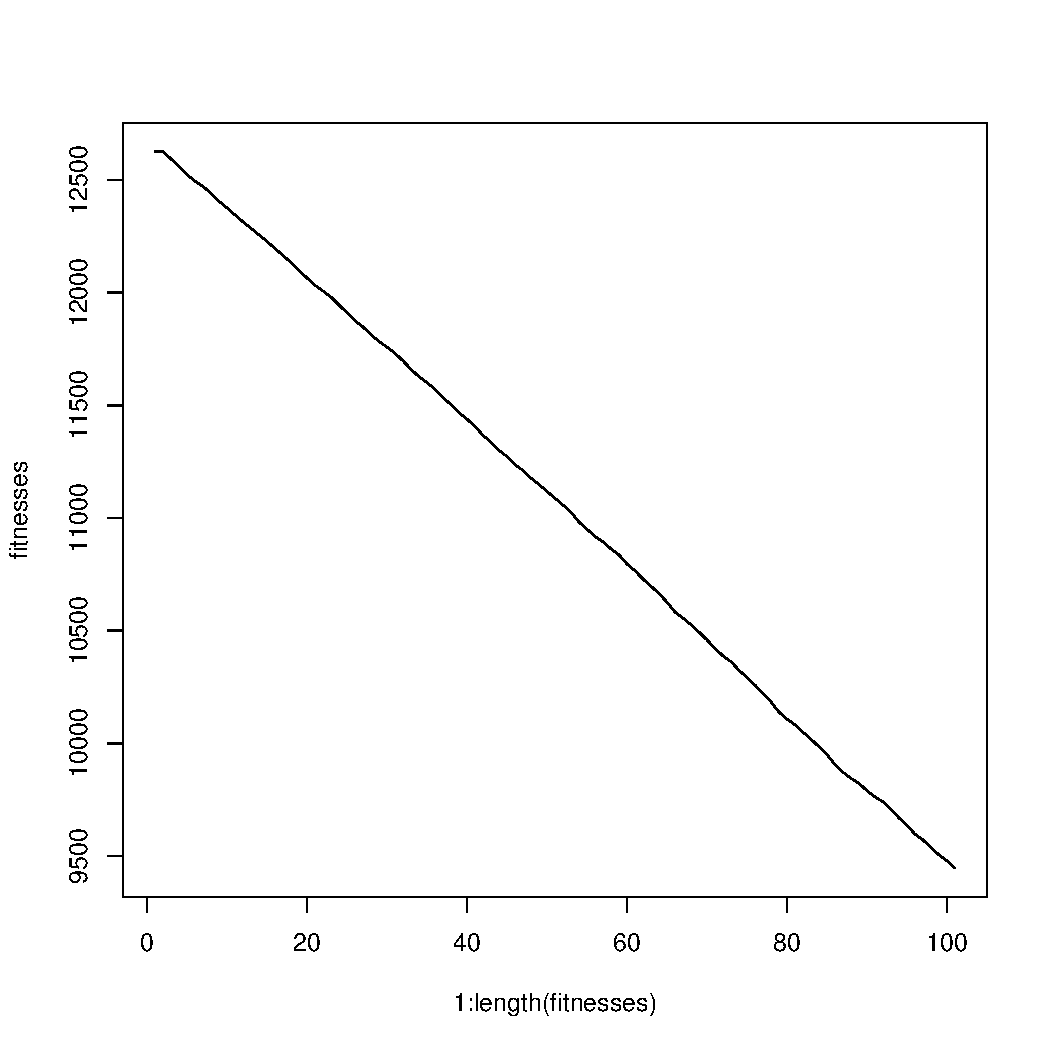
\includegraphics[width=60mm]{images/schwefel.ss/avg_101.pdf}
		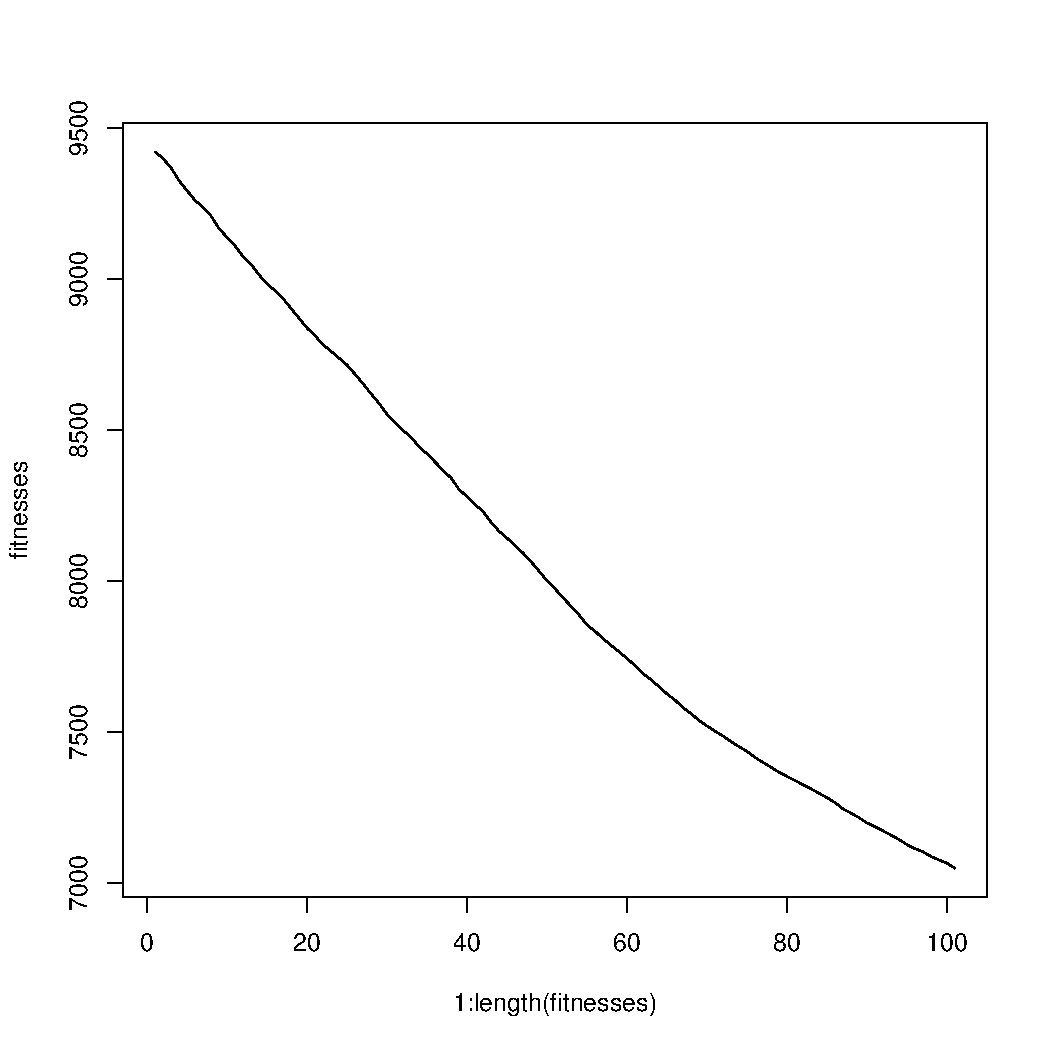
\includegraphics[width=60mm]{images/schwefel.ss/avg_202.pdf}
		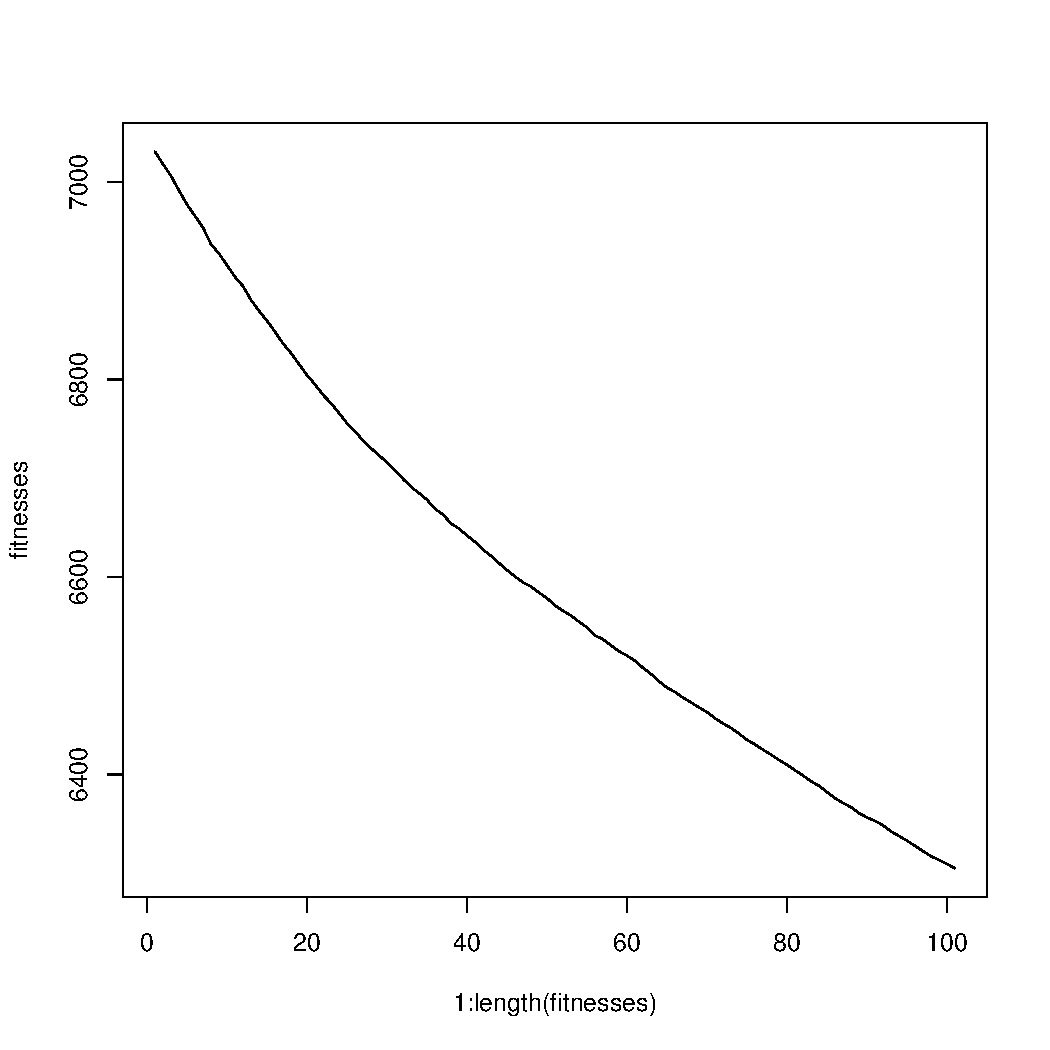
\includegraphics[width=60mm]{images/schwefel.ss/avg_303.pdf}
		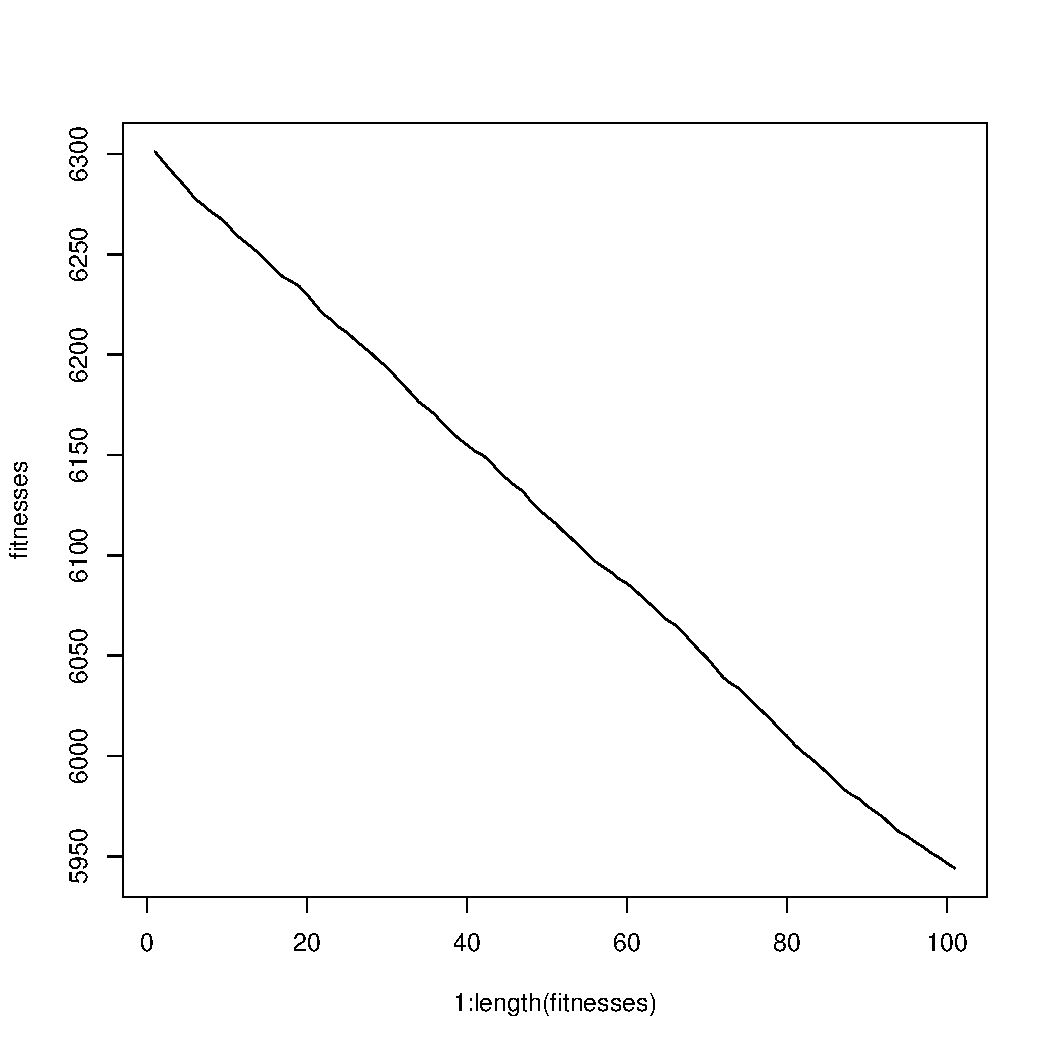
\includegraphics[width=60mm]{images/schwefel.ss/avg_404.pdf}
               	\caption{Average population fitnesses at 100, 202, 303, and 404 iterations, respectively, at 100 iteration wide snapshots}
                \label{schwefel_ss_avg_pop_fit}
        \end{center}
\end{figure}


\pagebreak

\section{Ackley}
\begin{figure}[!h]
        \begin{center}
		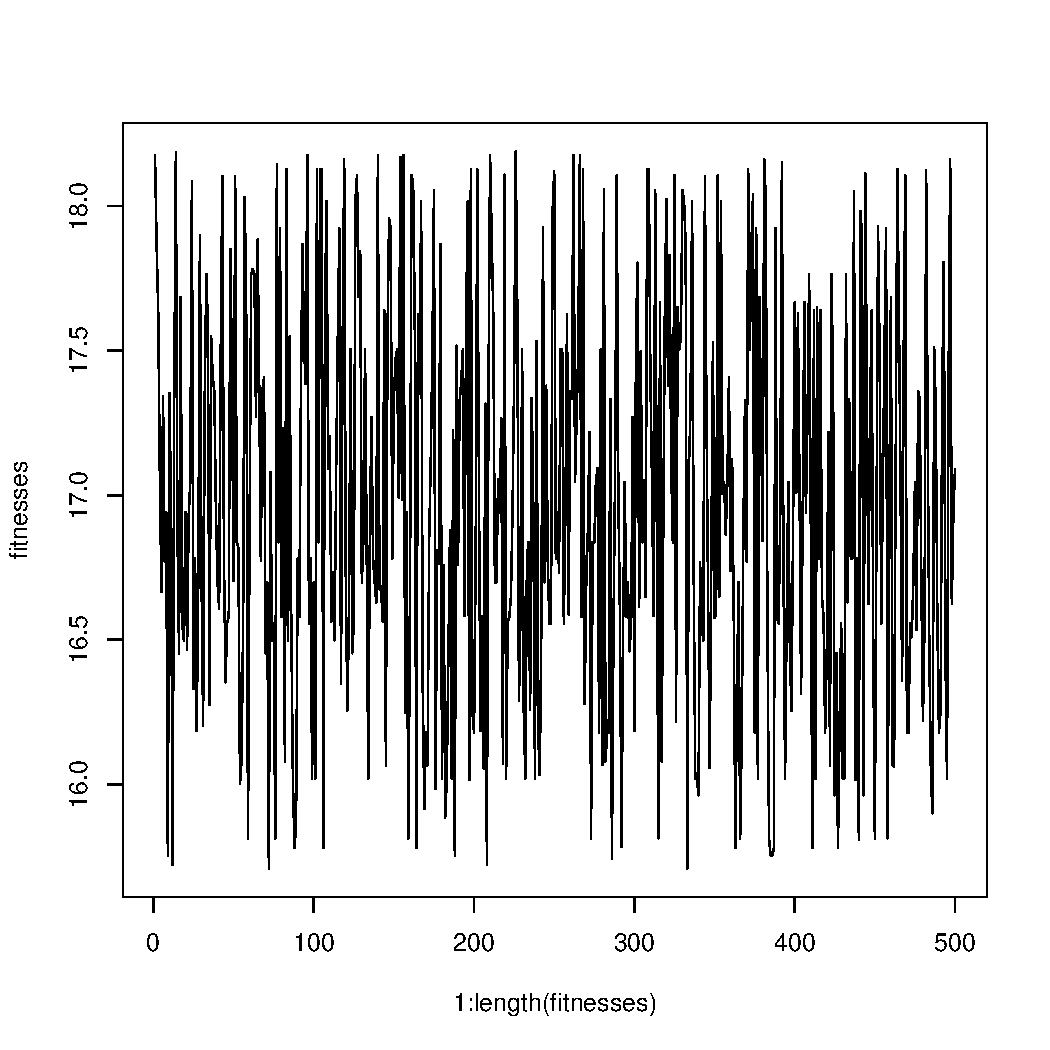
\includegraphics[width=60mm]{images/ackley.ss/ind_202.pdf}
		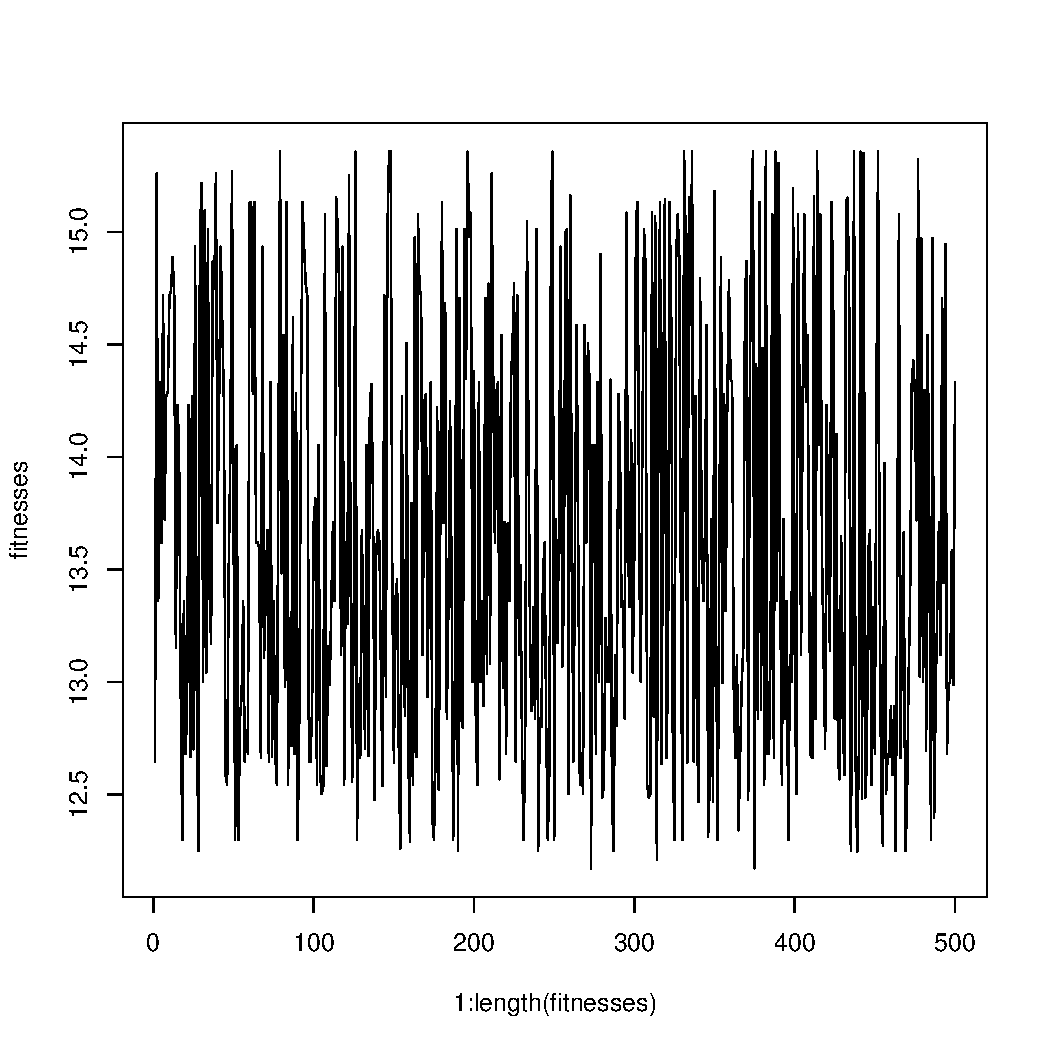
\includegraphics[width=60mm]{images/ackley.ss/ind_404.pdf}
		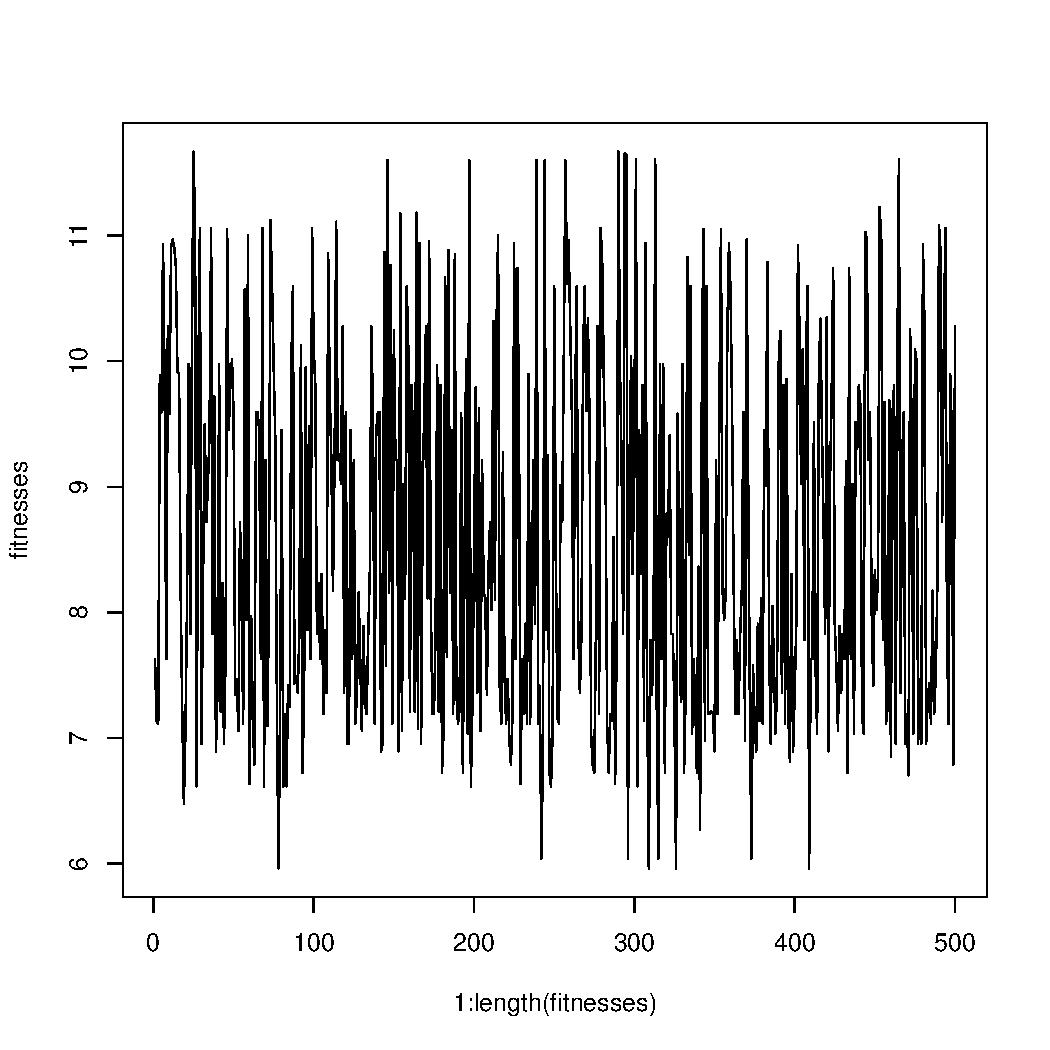
\includegraphics[width=60mm]{images/ackley.ss/ind_606.pdf}
		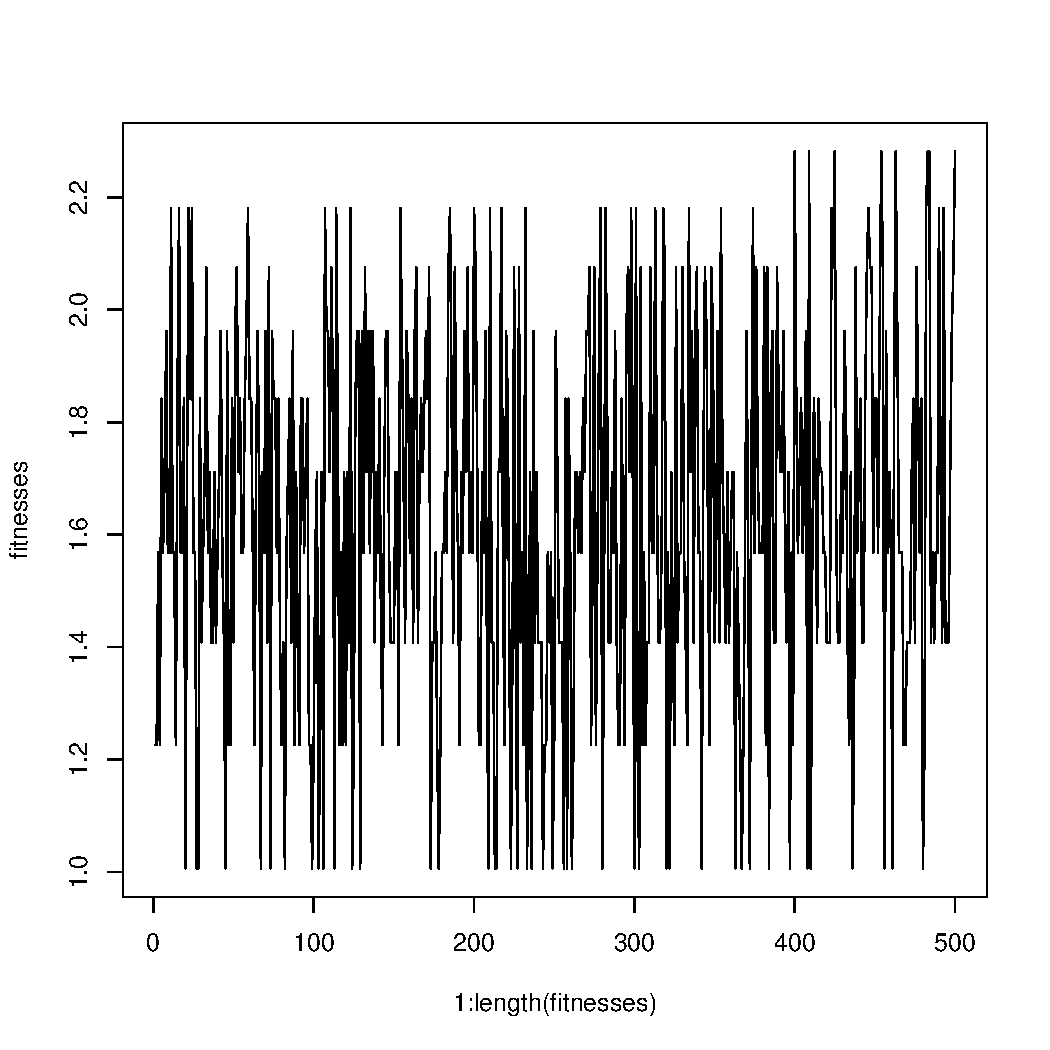
\includegraphics[width=60mm]{images/ackley.ss/ind_1010.pdf}
               	\caption{Population fitnesses at 100, 707, 1010, and 1010 iterations, respectively}
                \label{ackley_ss_pop_fit}
        \end{center}
\end{figure}

The Ackley steady state GA converged to 0.00 at 1151 generations (5 minutes 51 seconds), and right before converging, the lowest individual was:
\scriptsize
\begin{lstlisting}
[1] "1151  - Avg fitness: 0.984803584995115 min: 0.717124227444301 sd: 0.312872307329276"
 [1]  0  0  0  0  0  0  0  0  0  0  0 -1  0  0  0  0  0  0  0  0  0  0  0  0  0
[26]  0  0  0  0  0
[1] "Min fitnesses: 0"
[1] "Re-gen time: 0.505999999999972"
\end{lstlisting}
\normalsize

\pagebreak

\begin{figure}[!h]
        \begin{center}
		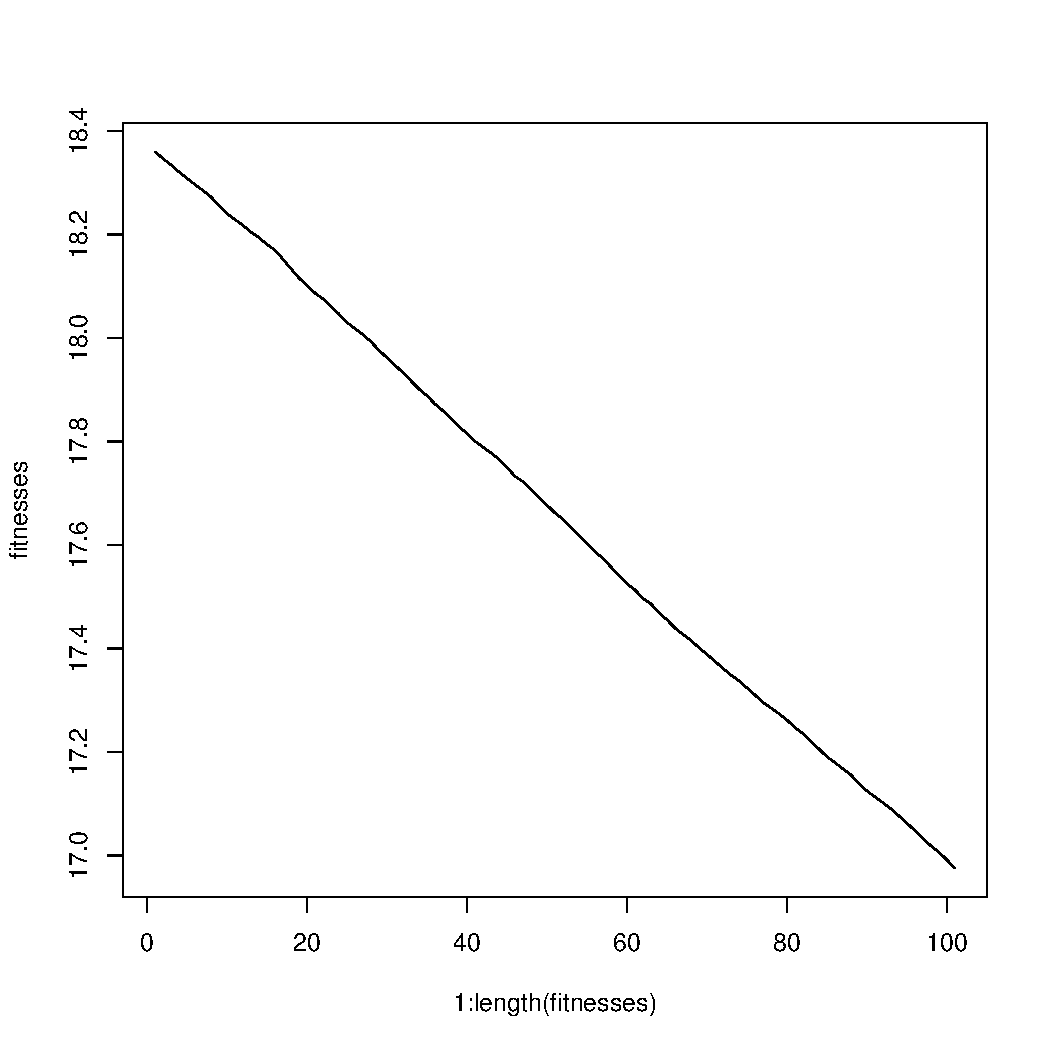
\includegraphics[width=60mm]{images/ackley.ss/avg_202.pdf}
		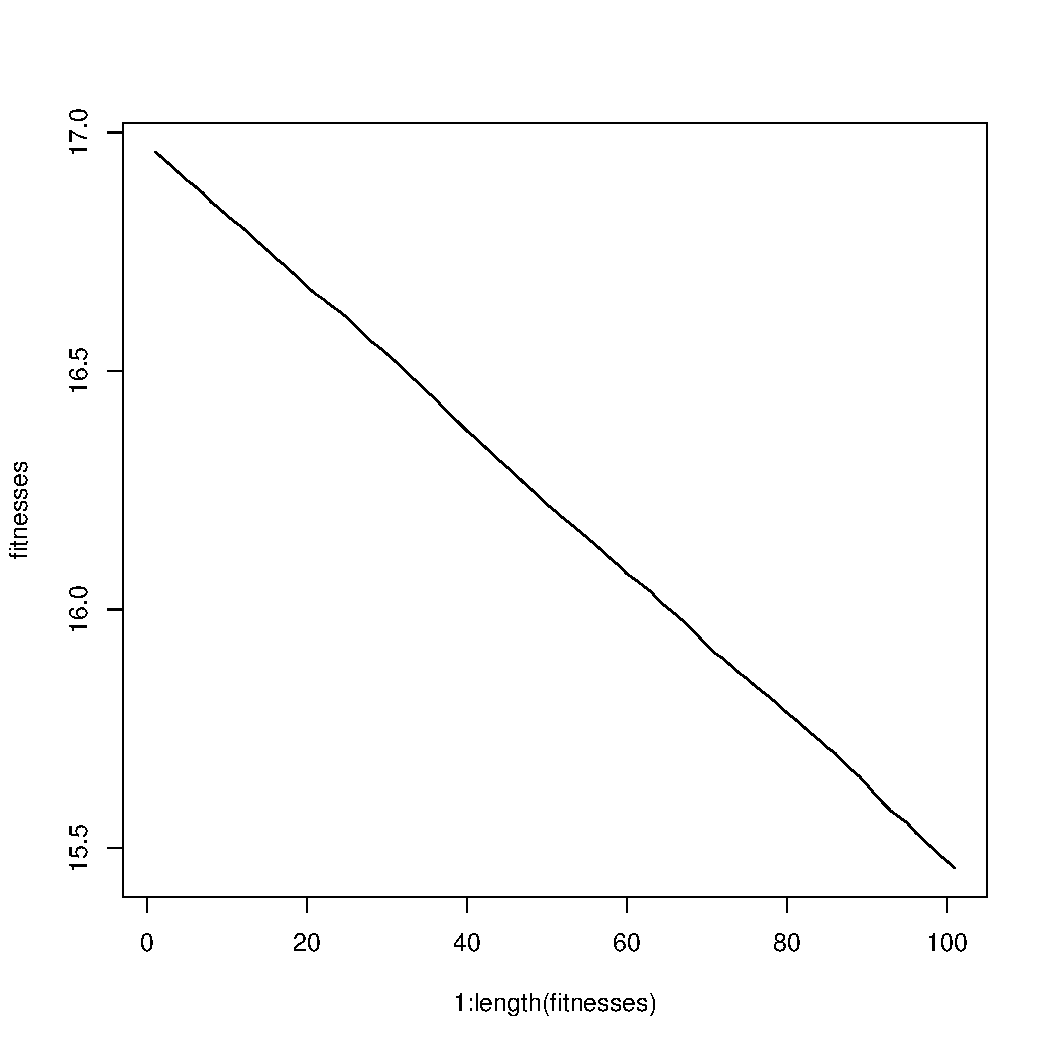
\includegraphics[width=60mm]{images/ackley.ss/avg_303.pdf}
		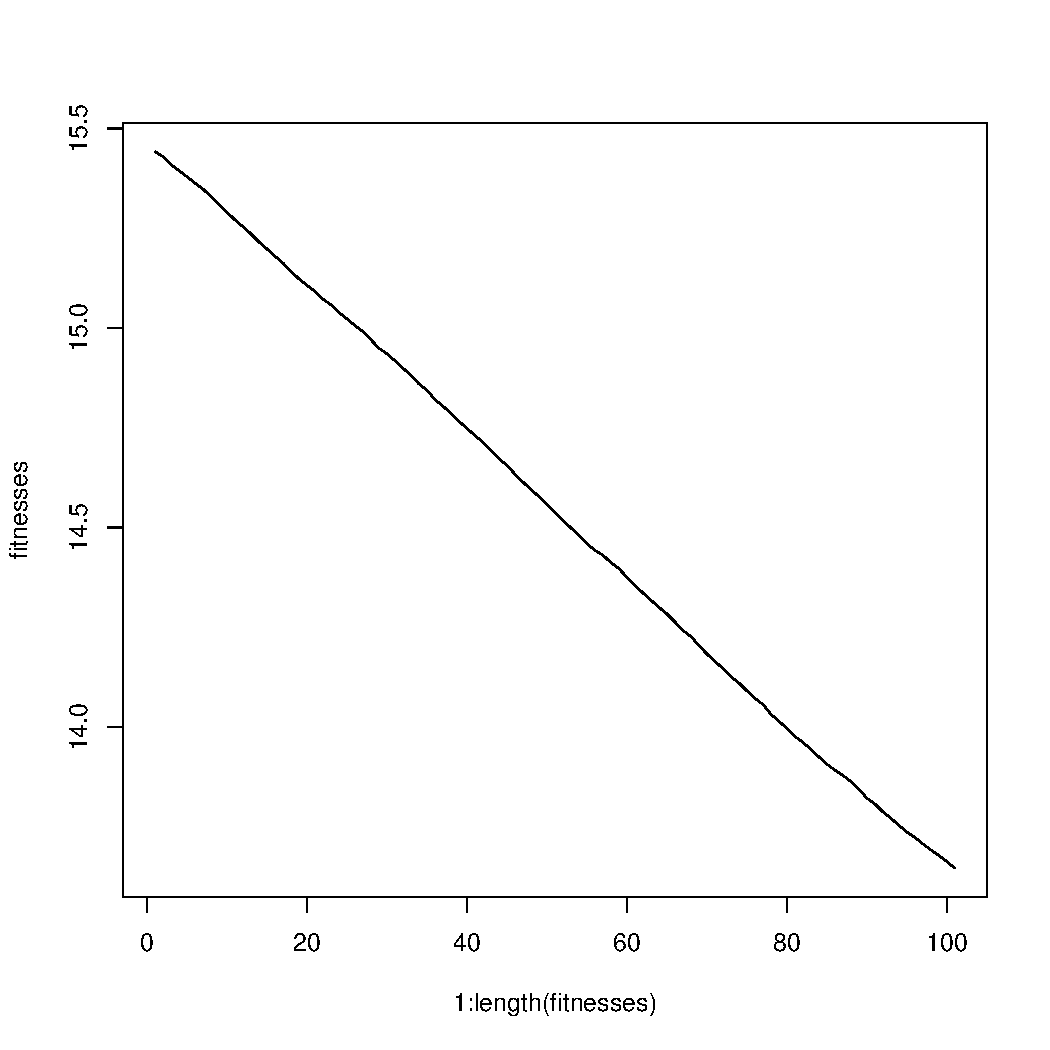
\includegraphics[width=60mm]{images/ackley.ss/avg_404.pdf}
		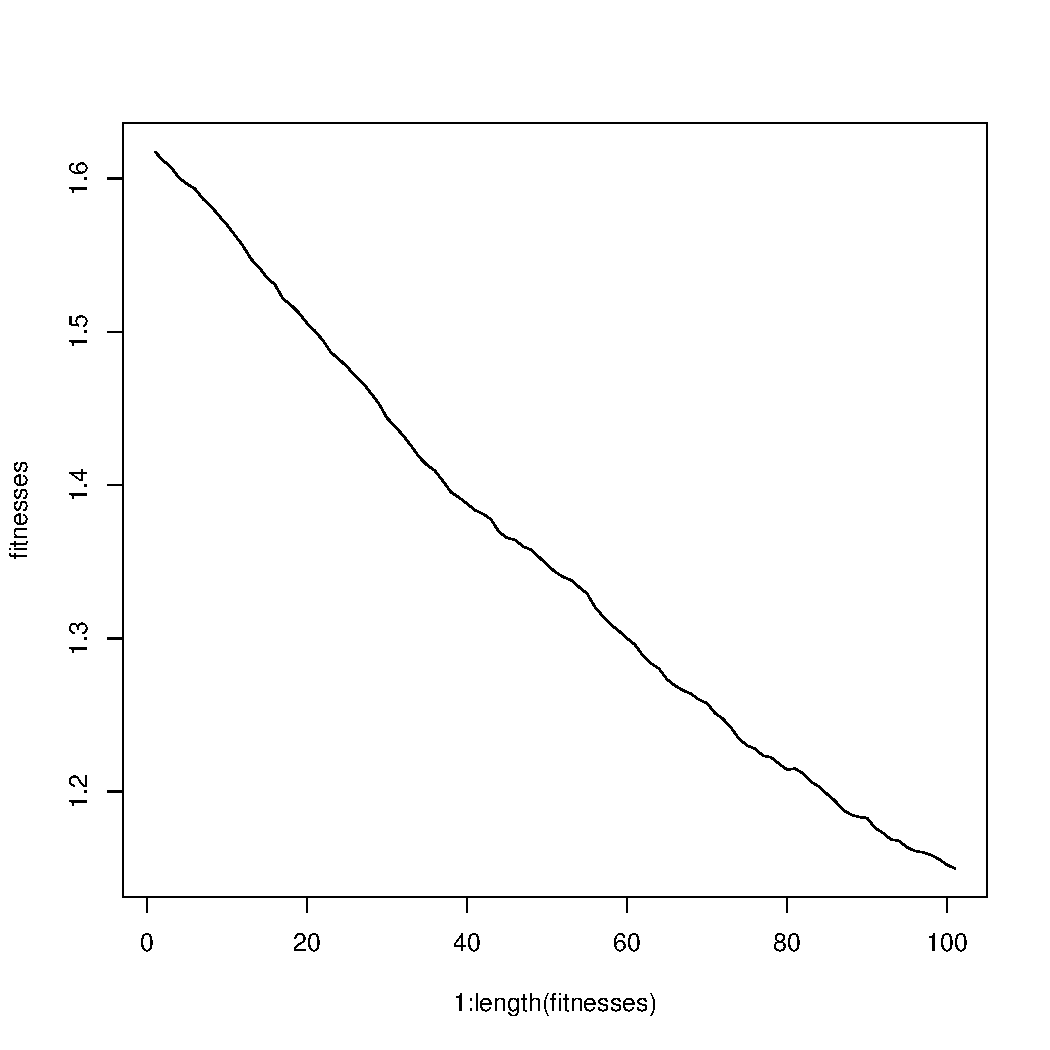
\includegraphics[width=60mm]{images/ackley.ss/avg_1111.pdf}
               	\caption{Average population fitnesses at 100, 202, 303, and 404 iterations, respectively, at 100 iteration wide snapshots}
                \label{ackley_ss_avg_pop_fit}
        \end{center}
\end{figure}


\pagebreak

\section{Griewangk}
\begin{figure}[!h]
        \begin{center}
		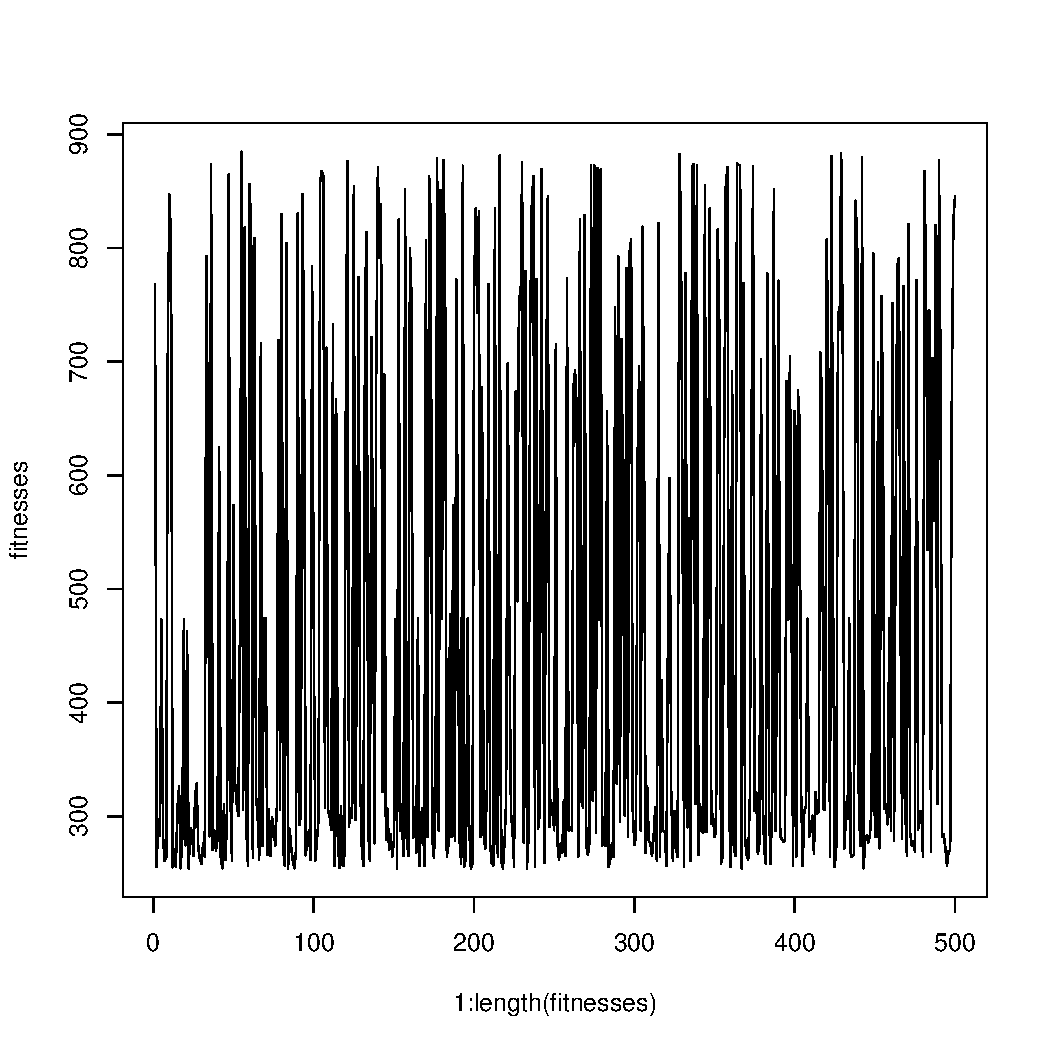
\includegraphics[width=60mm]{images/griewangk.ss/ind_101.pdf}
		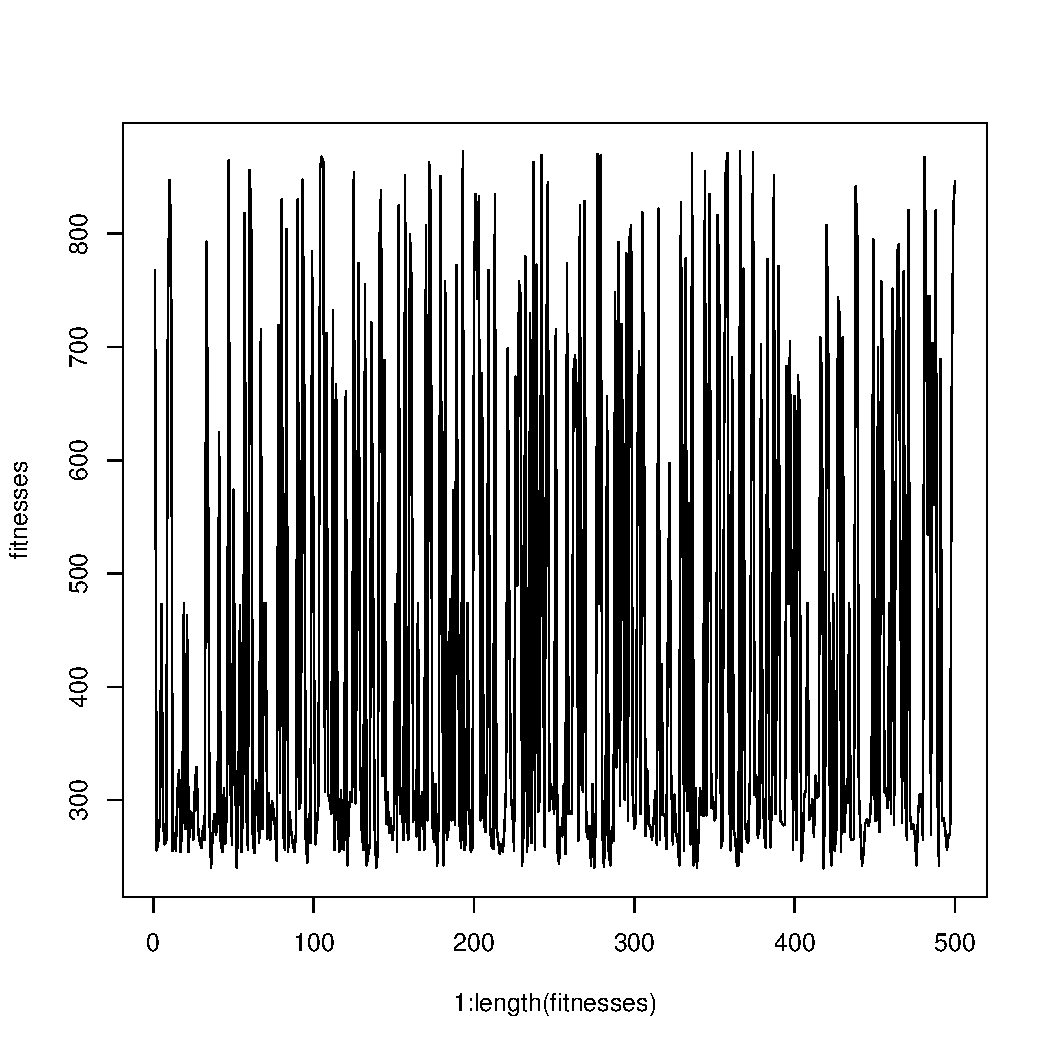
\includegraphics[width=60mm]{images/griewangk.ss/ind_110.pdf}
		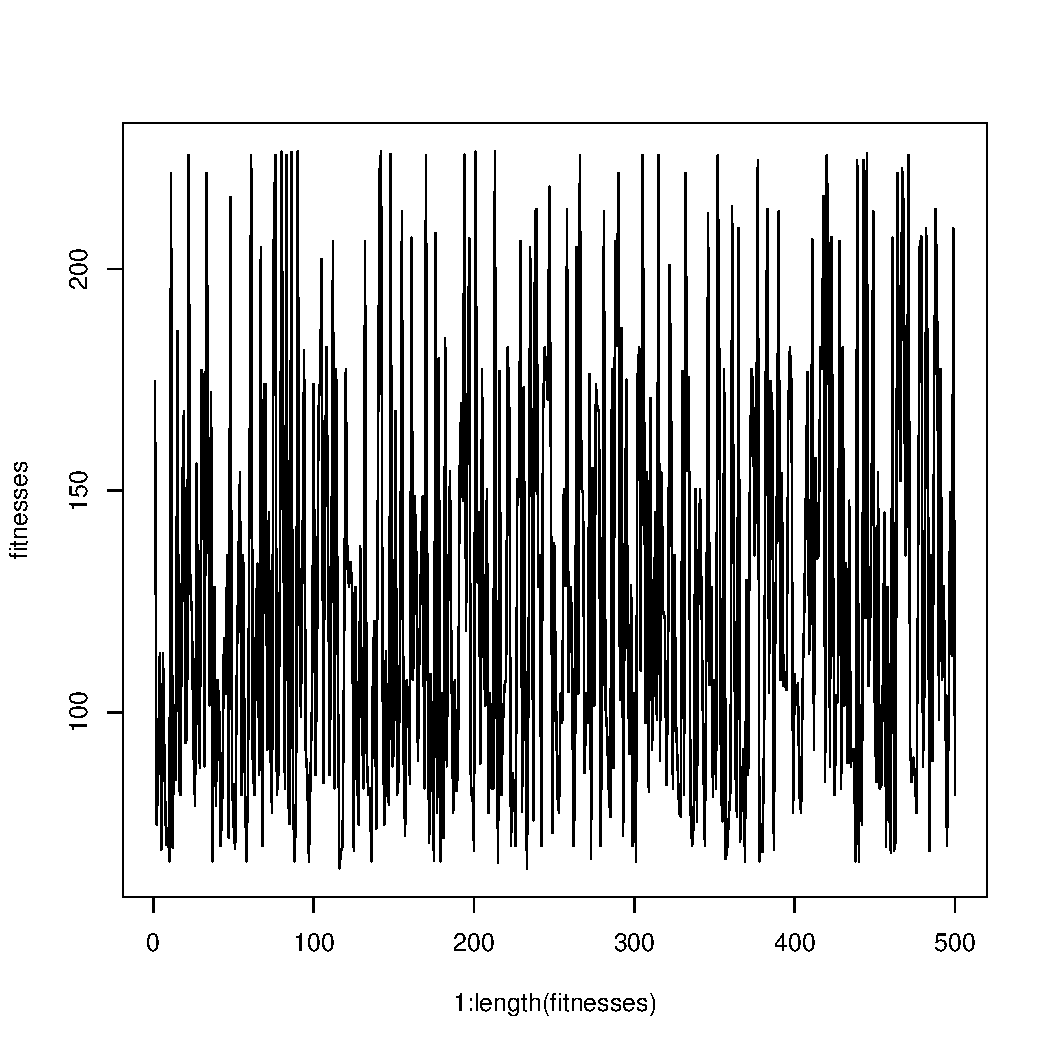
\includegraphics[width=60mm]{images/griewangk.ss/ind_303.pdf}
		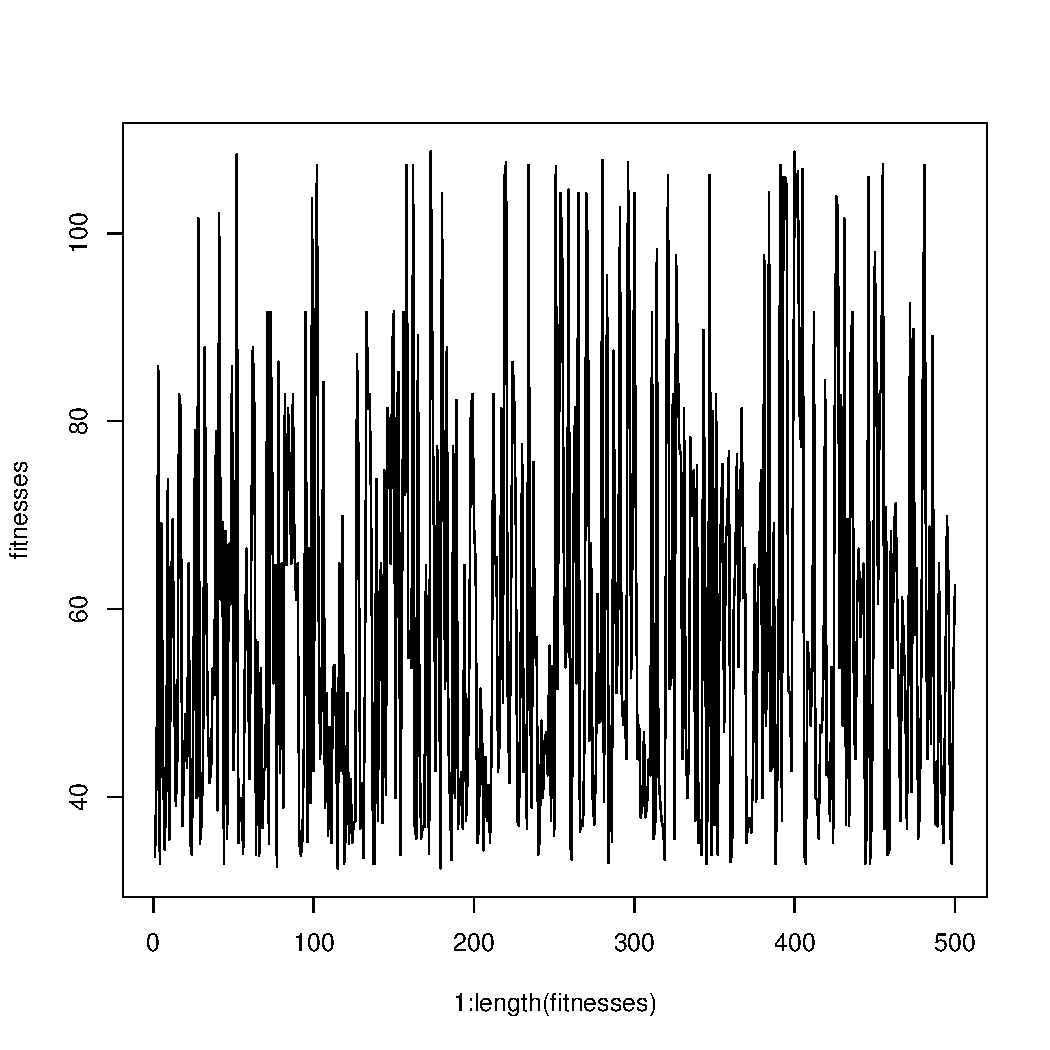
\includegraphics[width=60mm]{images/griewangk.ss/ind_404.pdf}
               	\caption{Population fitnesses at 100, 110, 303, and 404 iterations, respectively}
                \label{griewangk_ss_pop_fit}
        \end{center}
\end{figure}

The Griewangk steady state GA never converged to 0.00 (16 minutes 57 seconds), and at 10,000 generations, the lowest individual was:
\scriptsize
\begin{lstlisting}
[1] "10000  - Avg fitness: 1.33522979281519 min: 0.95813840335565 sd: 0.283156395057589"
[1]  0 -1 -1 -1 -1  1 -1 -2 -1  1  1  2  0 -2  2  2 -2 -1  1  4 -1 -1 -1 -1  1
[26]  0 -3 -1  1  0
[1] "Min fitnesses: 0.95813840335565"
[1] "Re-gen time: 0.184999999999945"
\end{lstlisting}
\normalsize

\pagebreak

\begin{figure}[!h]
        \begin{center}
		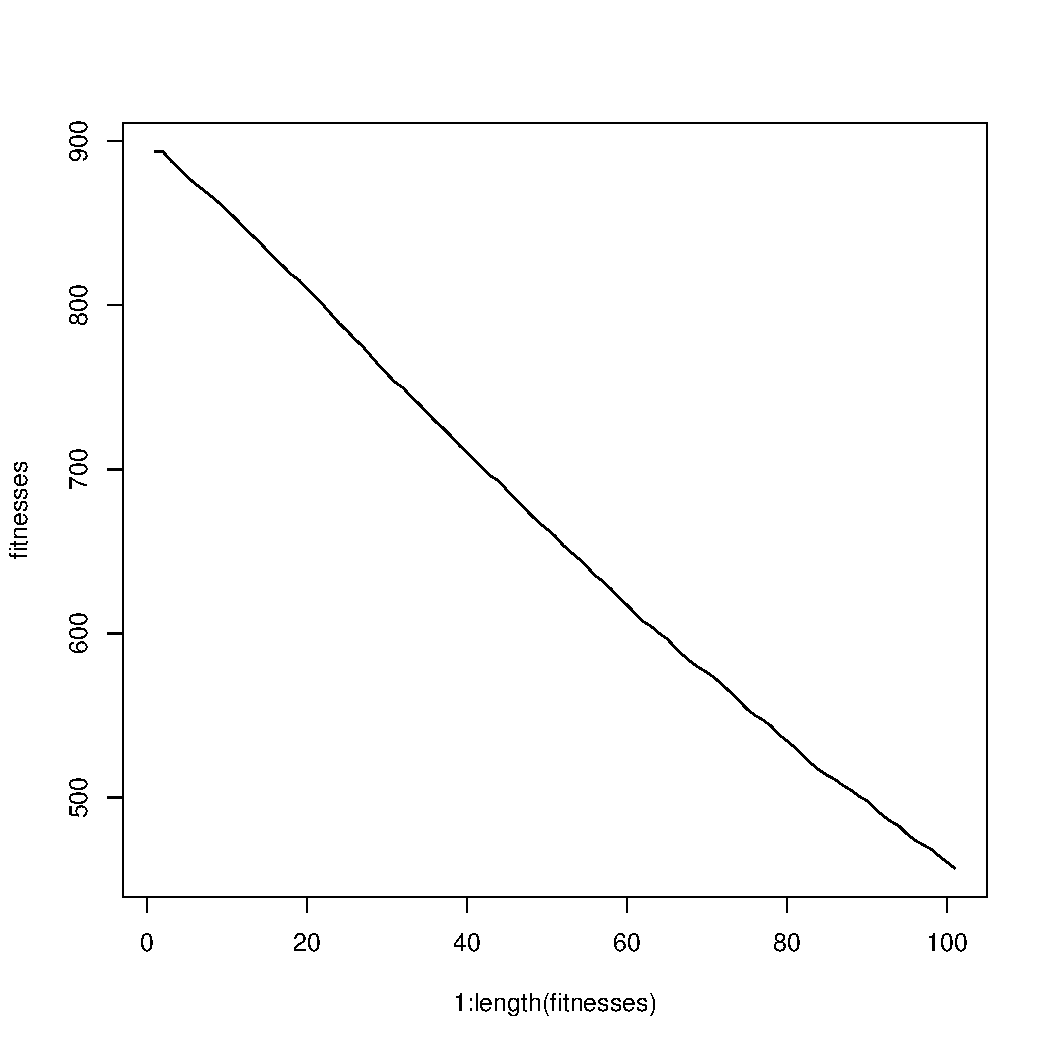
\includegraphics[width=60mm]{images/griewangk.ss/avg_101.pdf}
		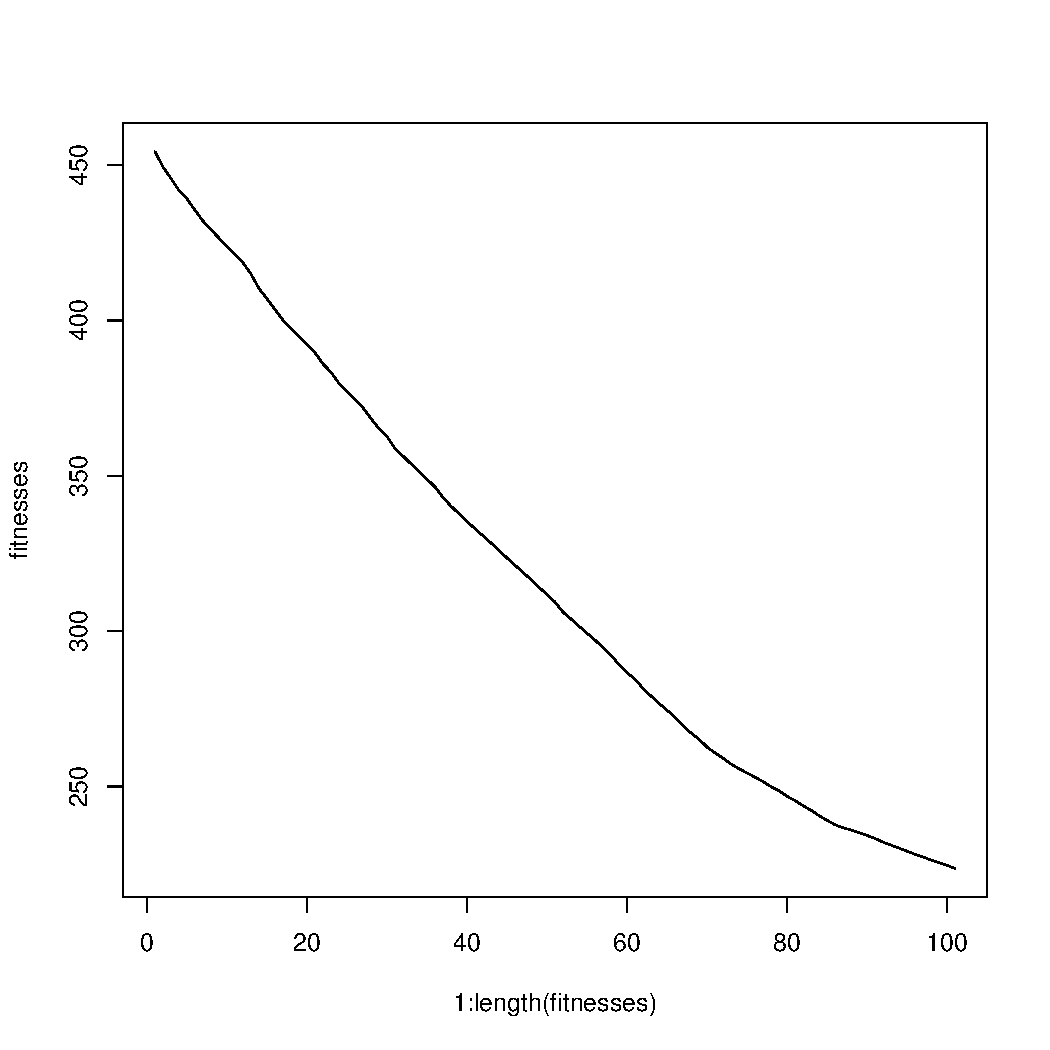
\includegraphics[width=60mm]{images/griewangk.ss/avg_202.pdf}
		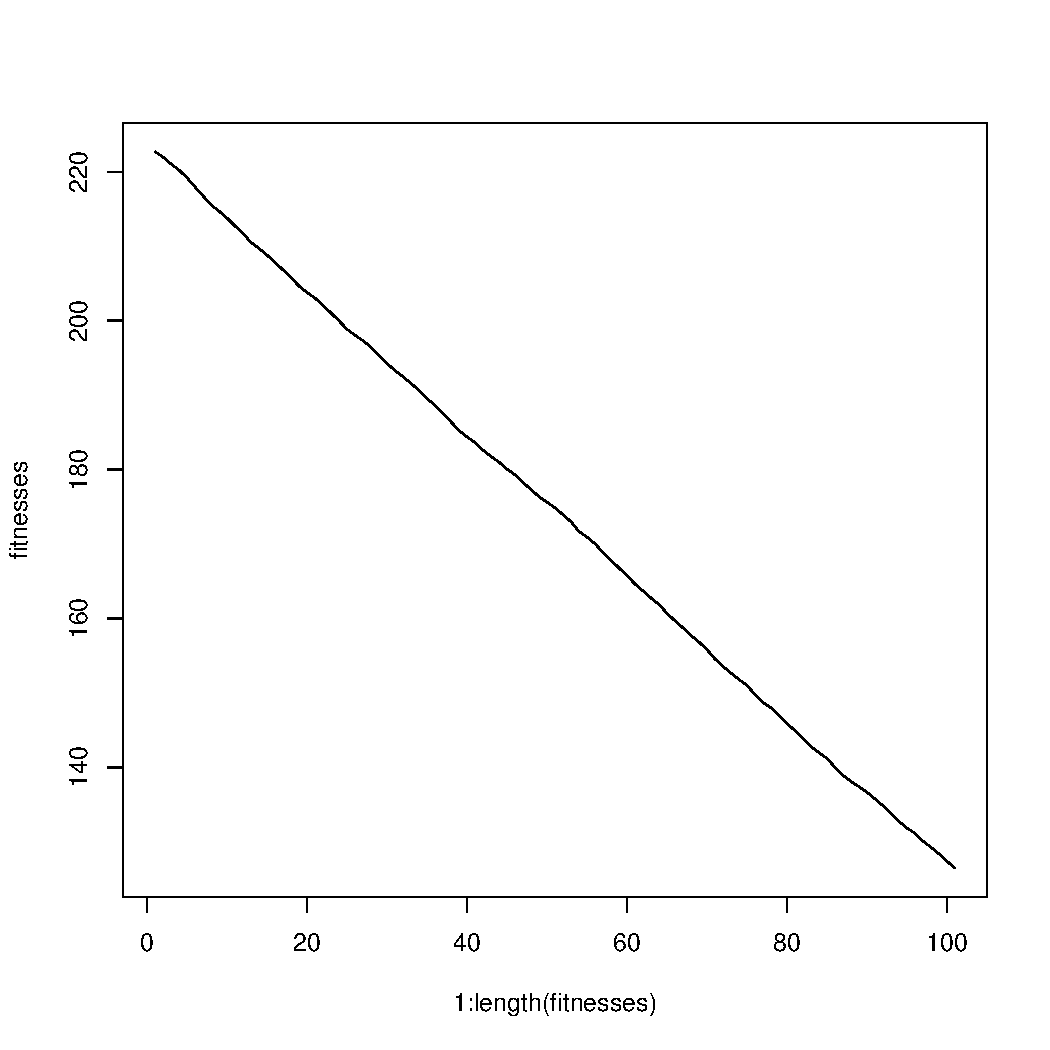
\includegraphics[width=60mm]{images/griewangk.ss/avg_303.pdf}
		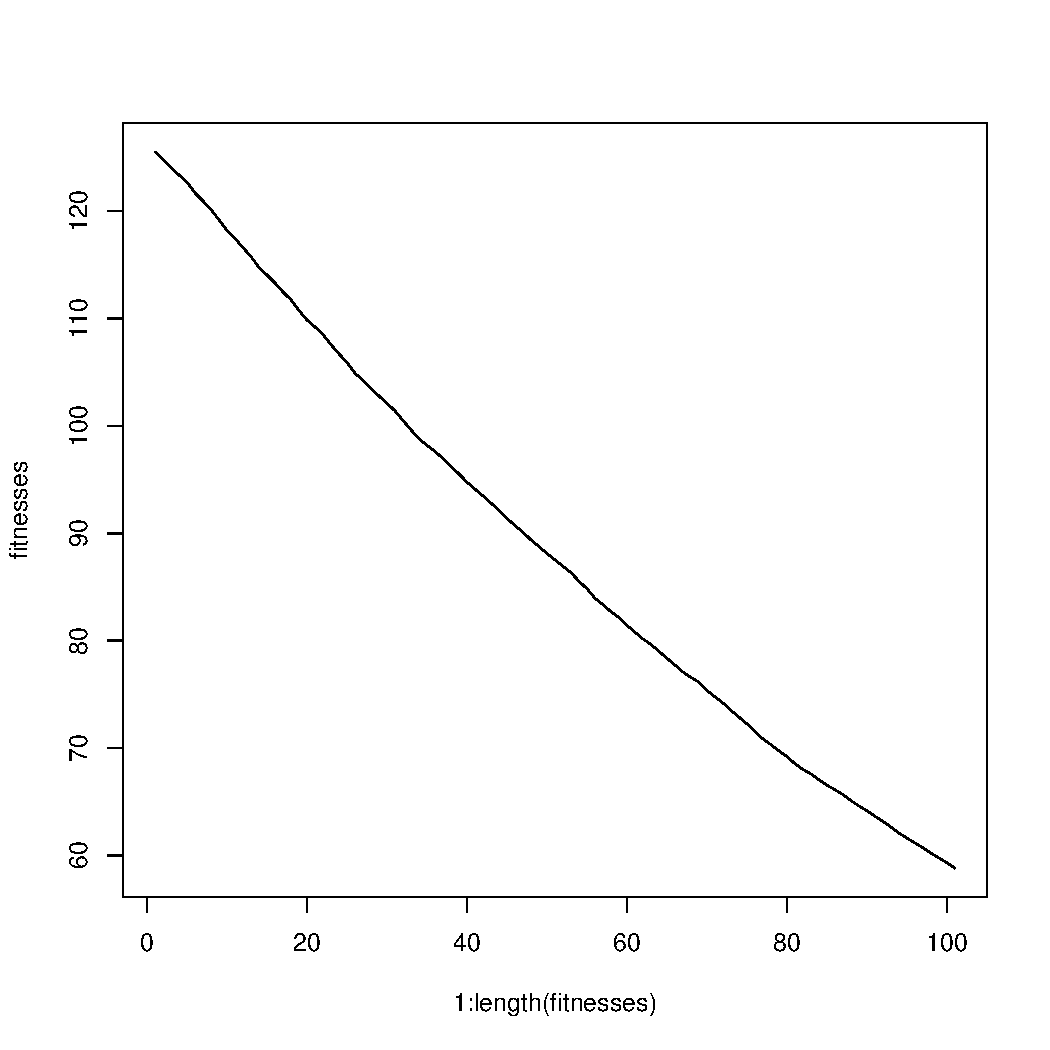
\includegraphics[width=60mm]{images/griewangk.ss/avg_404.pdf}
               	\caption{Average population fitnesses at 100, 202, 303, and 404 iterations, respectively, at 100 iteration wide snapshots}
                \label{griewangk_ss_avg_pop_fit}
        \end{center}
\end{figure}



\part{Conclusion}
\section{Algorithms}
\textbf{Steady state} preserves existing populations, which allows for more individual variance. This did better for this report than generational for the functions that had lots of local minimums. This was the case for all the functions, except the \textbf{spherical function}. The spherical function did better using a generational GA with elitism by about 7000 genertaions. But we applied the steady state GA for consistency.

The \textbf{ackley function} actually did the best, over spherical. The $ k $ and $ S $ parameters seemed well tuned for it, and the convergence was fairly steady towards down. It also did better than most of the other functions, in that it converged completely

The \textbf{rosenbrock function} did not converge, although its values got closer than the other functions. The function seemed to still be converging towards the end, so a higher $ S $ factor or $ k $ factor may have been needed.

The \textbf{griewangk function} never converged, although it too got reasonably close to converging. It also was still steadily converging during the end, so higher $ S $ or $ k $ factors would be good options to try to get convergence.

The \textbf{rastrigin function} never converged, although it had some good values. Overall, it didn't really get close. The function seemd to get stuck in a local minimum somewhere. Part of the problem could have been that the $ S $ factor was too big, so mutations didn't help it converge, at least locally. They could have helped get to a global, but didn't play a big enough factor


The \textbf{schwefel function} did very badly, although it did have some good values. Higher $ S $ and $ k $ values should definitely be tried. This would have been done actually, but I haven't better values so far, and ran out of time for more runs.


\end{document}
